\chapter{Measurement of Hadronic Production and $\Gamma(\psipp \rightarrow \nonDDbar)$}
\label{ch:non_DDbar}

The second part of the analysis concerns the measurement of hadronic events over the scan data energy region.
Using this information, we can extract the number of $\nonDDbar$ events found in data by subtracting all other known decay processes.
Comparing the found production rate of $\nonDDbar$ events to the previous measurement of $\xsecpsipptoDDbar$, we can then analyze the branching fraction of $\Gamma(\psipp \rightarrow \nonDDbar)$.


In order to determine the amount of hadronic events in the scan data region, we use continuum data taken at a lower energy (around \SI{3.650}{\GeV}).
This is due to complicated interactions in the region above the $\DDbar$ threshold which are currently not well modeled by our MC generators.
However, below the $\psip$, the process is more reliable.
If the production of hadronic events remains consistent over energy, we can use these measurements at lower energies to extract values at higher energies.

\section{Data and Monte Carlo Samples}
\label{sec:non_DDbar_data_samples}

\subsection{Data Samples}
\label{ssec:data_samples_non_DDbar}

The data used for this analysis was also produced by BEPCII and collected by BESIII.
The samples used include continuum data taken at \SI{3.650}{\GeV} in 2009 (old continuum), as well as multiple other continuum points taken around this energy in 2013 (new continuum).
We also use Round 1 (R1) and Round 2 (R2) of the high-statistics $\psipp$ data taken in 2010 and 2011, respectively.
Each of these samples, and their measured luminosities, can be seen in \Cref{tab:data_samples_non_DDbar}.
The values of luminosity were measured during a previous version of this analysis using the procedure described in \Cref{ssec:luminosity_measurement}.
The labels given to each continuum point are the intended energy targets, but may differ from their true values.
In addition to these datasets, the scan data described previously (\Cref{ssec:data_samples}) is also used.


\subsection{Center-of-Mass Energy Measurement}
\label{ssec:energy_measurement_non_DDbar}

As before, a precise measurement of each energy point is vital to the accuracy of the final results.
Most notably, due to the rapidly increasing shape of the $\psip$ cross section near the high end of the continuum points, the value of the 3671 (New) point has a dramatic effect on the $\qqbar$ extrapolation.
Following the procedure of \Cref{ssec:energy_measurement}, we measured the $\Ecm$ value of each continuum point.
This resulted in a \SIrange{4}{6}{\MeV} shift downwards for each of the new continuum points, but virtually no shift for the old continuum point.
The energy measurements are shown in \Cref{tab:data_samples_non_DDbar}.


\begin{table}[H]
\centering
\renewcommand\arraystretch{1.0}
\begin{tabular}{l|c r}
\hline
Sample Name & $\Ecm$ [\si{\GeV}] & Luminosity \si{\invpb} \\
\hline
3500 (New) & 3.496 & \num{  3.680 \pm 0.009} \\
3542 (New) & 3.538 & \num{  3.481 \pm 0.009} \\
3600 (New) & 3.596 & \num{  0.395 \pm 0.019} \\
3650 (New) & 3.644 & \num{  5.420 \pm 0.009} \\
3671 (New) & 3.665 & \num{  4.669 \pm 0.009} \\
3650 (Old) & 3.650 & \num{ 44.334 \pm 0.009} \\
3773 (R1)  & 3.773 & \num{926.922 \pm 0.092} \\
3773 (R2)  & 3.773 & \num{1978.92 \pm 0.091} \\
\hline
\end{tabular}
\caption{Data samples used for the inclusive measurement.}
{While the 3600 (New) sample was intended to be similar in luminosity to the other continuum points, accelerator issues inhibited the data collection procedure. 
The new continuum points also have a much smaller luminosity compared to the other datasets used in this analysis.}
\label{tab:data_samples_non_DDbar}
\end{table}


\section{Event Selection}
\label{sec:non_DDbar_event_selection}

In order to select the number of hadronic events in each sample, we apply a variety of cuts.
For charged tracks in the MDC, these include the cuts shown in \Cref{tab:charged_cuts_non_DDbar}.

\begin{table}[H]
\centering
\renewcommand\arraystretch{1.0}
\begin{tabular}{c| r@{$\; < \;$}l}
\hline
Vertex ($xy$) & $V_{xy}$ & \pp \SI{1}{\cm} \\
Vertex ($z$)  & $|Vz|$   & \SI{10}{\cm} \\
MDC Angle & $|\cos\theta|$ & 0.93 \\
\hline
\end{tabular}
\caption{Selection cuts on charged tracks used to count hadronic events.}
\label{tab:charged_cuts_non_DDbar}
\end{table}

For neutral tracks in the EMC, these include the cuts shown in \Cref{tab:neutral_cuts_non_DDbar}.

\begin{table}[H]
\centering
\renewcommand\arraystretch{1.0}
\begin{tabular}{c|l r}
\hline
Minimum Energy (Barrel) & $E_{\text{EMC}} > \SI{25}{\MeV}$ & $(|\cos\theta| < 0.80)$ \\
Minimum Energy (Endcap) & $E_{\text{EMC}} > \SI{50}{\MeV}$ & $(0.86 < |\cos\theta| < 0.92)$ \\
TDC Timing & $(0 \leq t \leq 14) \times \SI{50}{\ns}$ & \\
\hline
\end{tabular}
\caption{Selection cuts on neutral tracks used to count hadronic events.}
\label{tab:neutral_cuts_non_DDbar}
\end{table}


To reject background events of $\bhabha$ or $\ee \rightarrow \gamma\gamma$, we also employ cuts related to the most energetic and highest momentum tracks in the event.
These are listed in \Cref{tab:bhabha_cuts_non_DDbar}.

\begin{table}[H]
\centering
\renewcommand\arraystretch{1.0}
\begin{tabular}{l|l@{}l l@{}l}
\hline
\multirow{4}{*}{Highest Energy}   & $\cosmax_+ <  $ & 0.8                            & \multirow{2}{*}{($\Ntrk$} & \multirow{2}{*}{ = 2)} \\
                                  & $\cosmax_- > -$ & 0.8                            & & \\
\cline{2-5}
                                  & $\cosmax_+ <  $ & 0.8 or $\pEmax_+ \leq 0.3$     & \multirow{2}{*}{($\Ntrk$} & \multirow{2}{*}{ = 3, 4)} \\
                                  & $\cosmax_- > -$ & 0.8 or $\pEmax_- \leq 0.3$     & & \\
\hline
\multirow{2}{*}{Highest Momentum} & \multicolumn{2}{l}{$0.8 \leq \Epmax_+ \leq 1.1$} & & \\
                                  & \multicolumn{2}{l}{$0.8 \leq \Epmax_- \leq 1.1$} & & \\
\hline
\end{tabular}
\caption{Selection cuts to remove Bhabha and two-photon backgrounds.}
{The $_+$ and $_-$ denote positively and negatively charged tracks, respectively.  The $^{\text{max}}$ notation indicates the highest energy or momenta track for the corresponding charge.  The energy cuts depend on the total number of charged tracks in the event, $\Ntrk$.}
\label{tab:bhabha_cuts_non_DDbar}
\end{table}

After applying these sets of cuts, there are three groups of cuts which are considered: Standard (SHAD), Loose (LHAD), and Tight (THAD).
For the nominal procedure, SHAD is used, while LHAD and THAD are for systematic consideration.
The cuts included in each of these sets are shown in \Cref{tab:shad_cuts_non_DDbar,tab:lhad_cuts_non_DDbar,tab:thad_cuts_non_DDbar}.
These apply to the number of charged tracks ($\Ntrk$), the visible energy ($\Evis$), the total visible momentum in the $z$-direction ($\pzvistot$), the maximum shower energy ($\Eemcmax$), and the total shower energy ($\Eemctot$).
Here, `visible' refers to the sum over charged and neutral tracks.

\begin{table}[H]
\centering
\renewcommand\arraystretch{1.0}
\begin{tabular}{l|r@{ }l l}
\hline
Number of Tracks                     & $\Ntrk$ & $ > 2$               &                  \\
\hline
Visible Energy                       & $\EvisE$ & $ > 0.3$            &                  \\
\hline
Visible Momentum                     & $\pzEvis$ & $ < 0.6$           & $(\Ntrk = 3, 4)$ \\
\hline
Maximum Shower Energy                & $\EemcEmax$ & $ < 0.75$           & $(\Ntrk = 3, 4)$ \\
\hline
\multirow{2}{*}{Total Shower Energy} & \multicolumn{2}{c}{$0.25 < \EemcEtot < 0.75$} & $(\Ntrk = 3)$ \\
                                     & \multicolumn{2}{c}{$0.15 < \EemcEtot < 0.75$} & $(\Ntrk = 4)$ \\
\hline
\end{tabular}
\caption{Standard selection cuts (SHAD) for counting hadronic events.}
\label{tab:shad_cuts_non_DDbar}
\end{table}

\begin{table}[H]
\centering
\renewcommand\arraystretch{1.0}
\begin{tabular}{l|r@{ }l l}
\hline
Number of Tracks                       & $\Ntrk$ & $ > 1$               &                  \\
\hline
\multirow{2}{*}{Visible Energy}        & $\EvisE$ & $ > 0.4$            & $(\Ntrk = 2)$    \\
                                       & $\EvisE$ & $ > 0.3$            & $(\Ntrk \geq 3)$ \\
\hline                                 
\multirow{2}{*}{Visible Momentum}      & $\pzEvis$ & $ < 0.3$           & $(\Ntrk = 2)$    \\
                                       & $\pzEvis$ & $ < 0.6$           & $(\Ntrk = 3, 4)$ \\
\hline
\multirow{2}{*}{Maximum Shower Energy} & $\EemcEmax$ & $ < 0.50$           & $(\Ntrk = 2)$    \\
                                       & $\EemcEmax$ & $ < 0.75$           & $(\Ntrk = 3, 4)$ \\
\hline                                 
\multirow{2}{*}{Total Shower Energy}   & \multicolumn{2}{c}{$0.25 < \EemcEtot < 0.75$} & $(\Ntrk = 2, 3)$ \\
                                       & \multicolumn{2}{c}{$0.15 < \EemcEtot < 0.75$} & $(\Ntrk = 4)$    \\
\hline
\end{tabular}
\caption{Loose selection cuts (LHAD) for counting hadronic events.}
\label{tab:lhad_cuts_non_DDbar}
\end{table}

\begin{table}[H]
\centering
\renewcommand\arraystretch{1.0}
\begin{tabular}{l|r@{ }l l}
\hline
Number of Tracks                     & $\Ntrk$ & $ > 3$               &                  \\
\hline
Visible Energy                       & $\EvisE$ & $ > 0.4$            &                  \\
\hline
Visible Momentum                     & $\pzEvis$ & $ < 0.6$           & $(\Ntrk = 4)$ \\
\hline
Maximum Shower Energy                & $\EemcEmax$ & $ < 0.75$           & $(\Ntrk = 4, 5)$ \\
\hline
\multirow{2}{*}{Total Shower Energy} & \multicolumn{2}{c}{$0.15 < \EemcEtot < 0.75$} & $(\Ntrk = 4)$ \\
                                     & \multicolumn{2}{c}{$0.00 < \EemcEtot < 0.75$} & $(\Ntrk = 5)$ \\
\hline
\end{tabular}
\caption{Tight selection cuts (THAD) for counting hadronic events.}
\label{tab:thad_cuts_non_DDbar}
\end{table}

\section{Hadron Counting}
\label{sec:hadron_counting}

In order to determine the total number of hadronic events in each data sample, we use the average velocity in the $z$-direction.
Signal events should have tracks which average to zero around the collision point, while background events will have randomly oriented momenta.
The fits are done with a double Gaussian shape for the signal and a 2nd order polynomial for the background.

\begin{figure}[H]
\centering
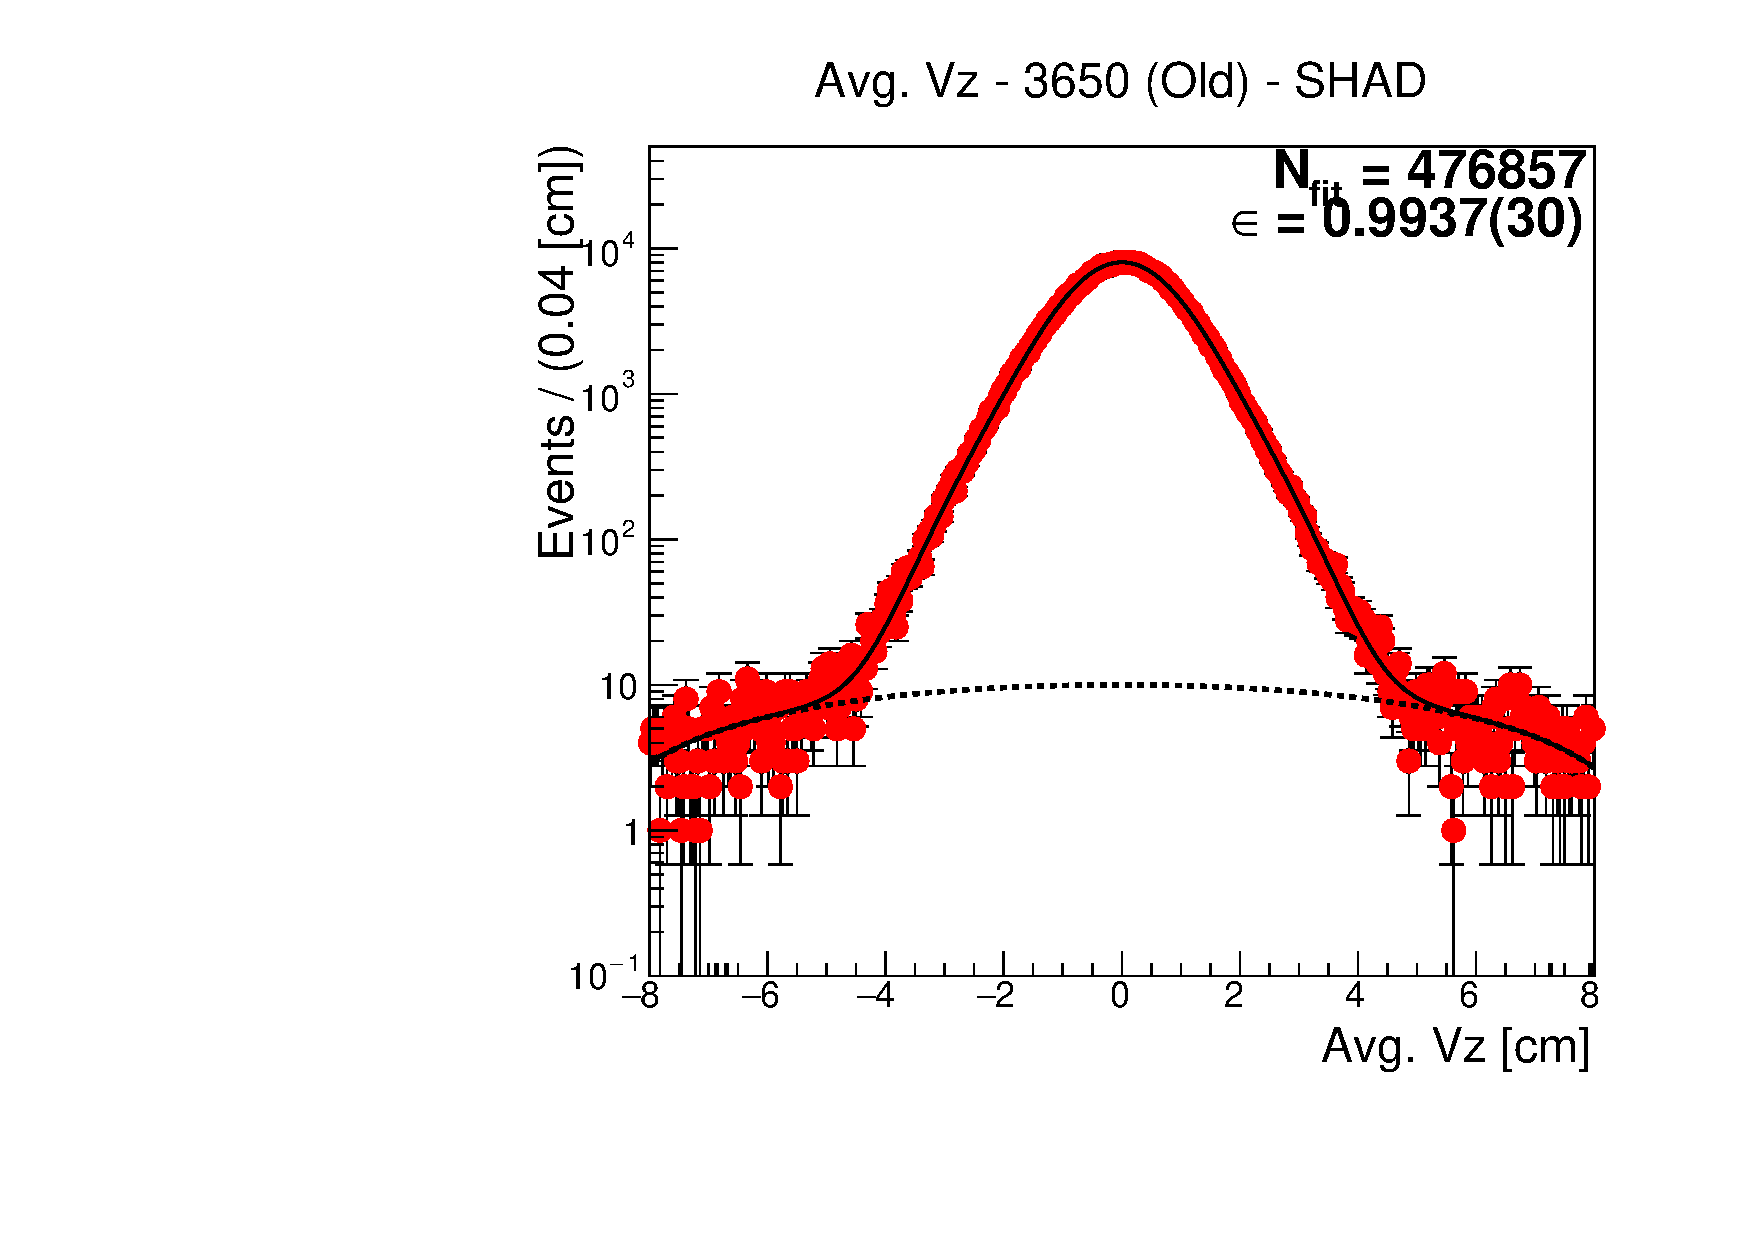
\includegraphics[scale=0.25]{figures/plots/nonDDbar_fit_results/3650_old/fit_old_3650_data_SHAD.pdf}
\hspace{-0.5cm}
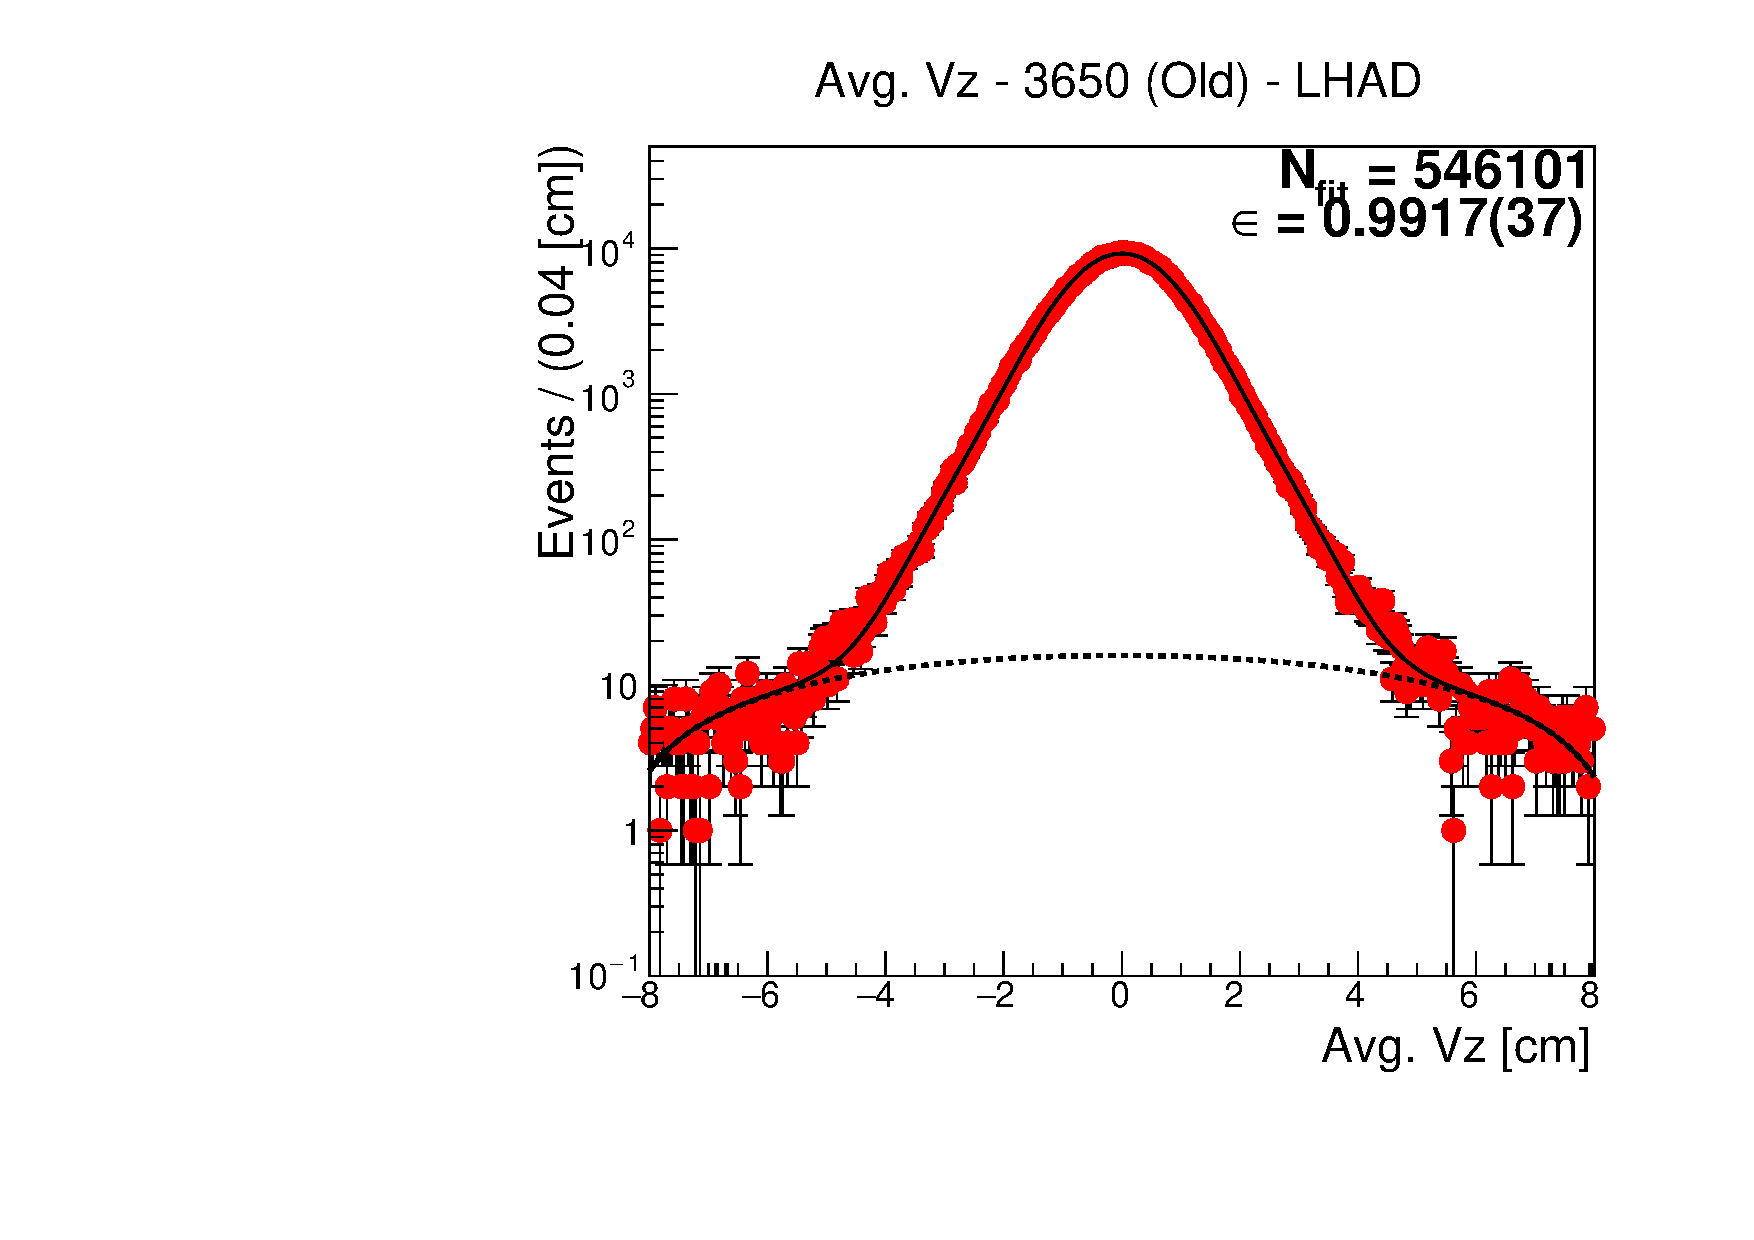
\includegraphics[scale=0.25]{figures/plots/nonDDbar_fit_results/3650_old/fit_old_3650_data_LHAD.pdf}
\hspace{-0.5cm}
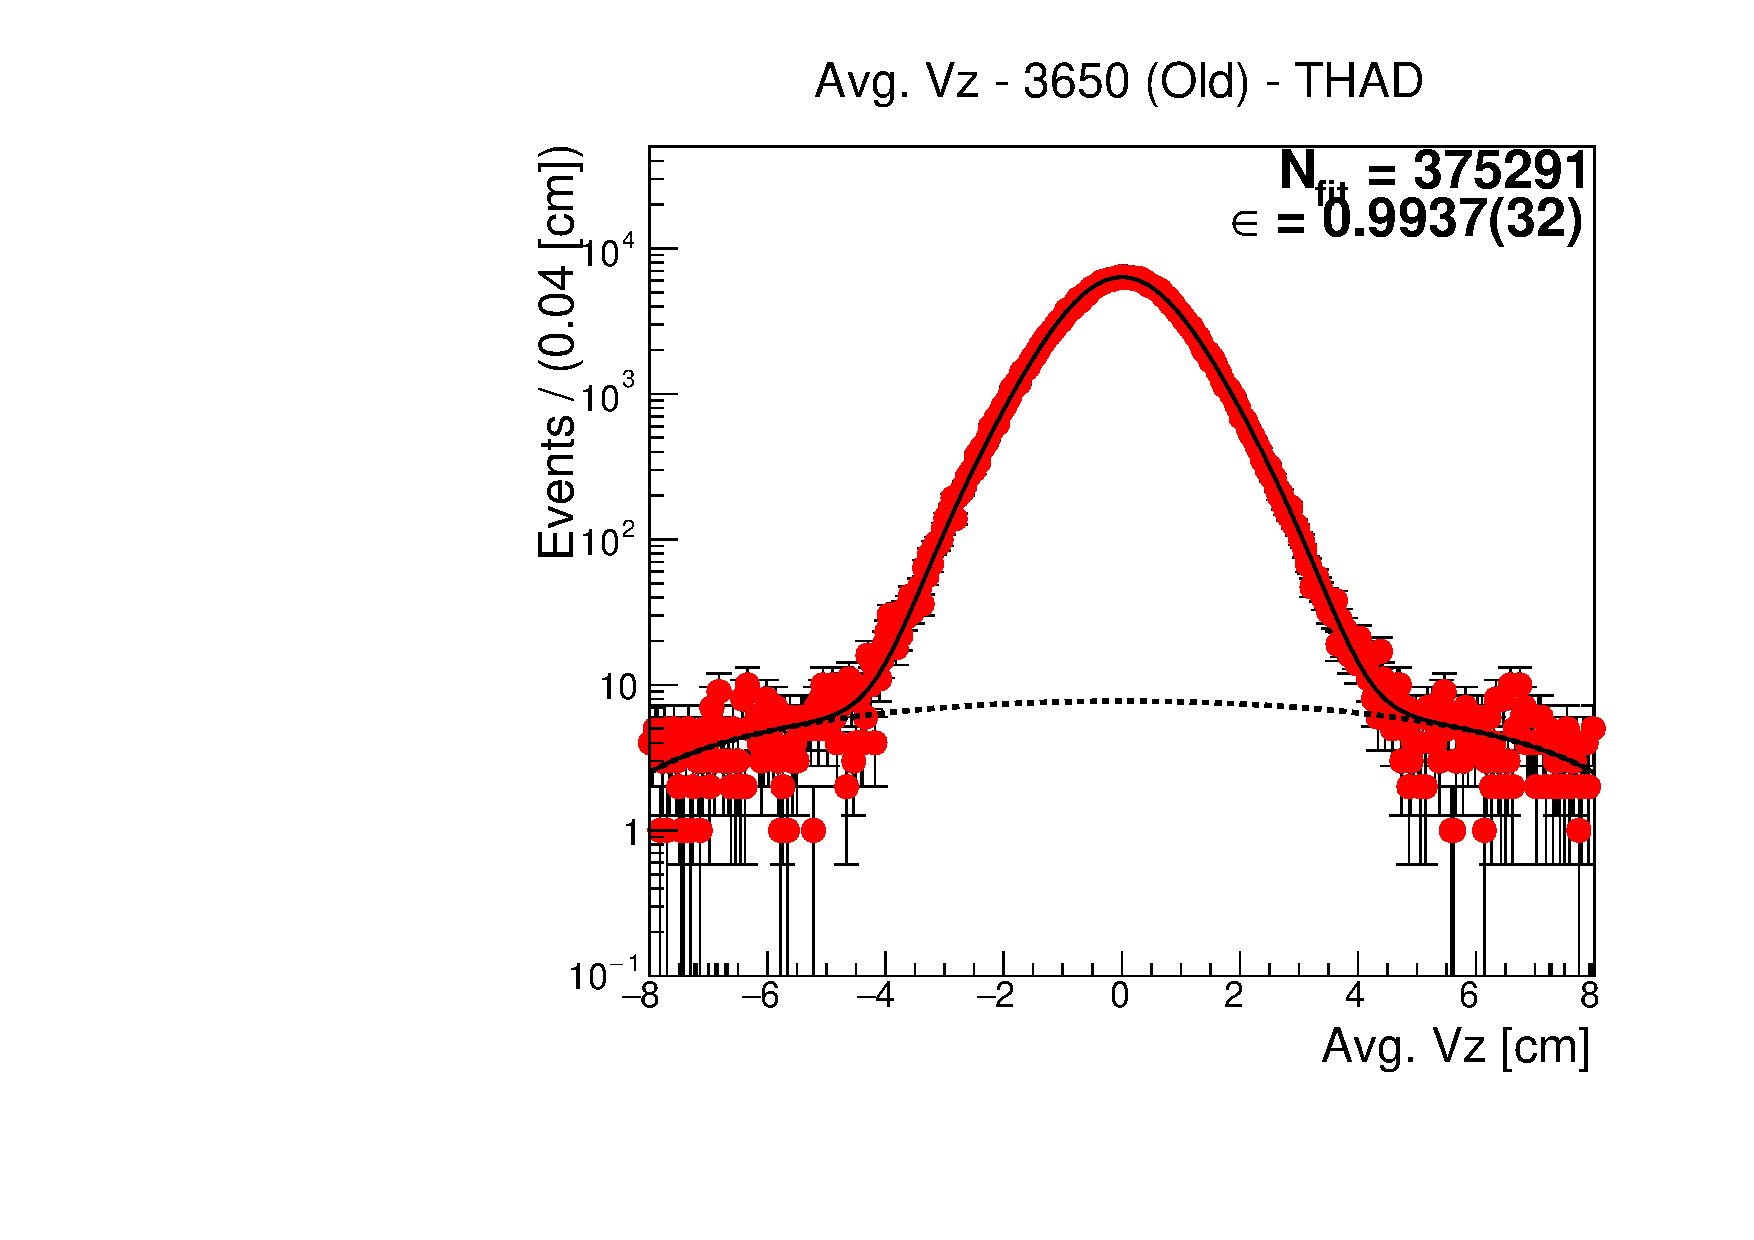
\includegraphics[scale=0.25]{figures/plots/nonDDbar_fit_results/3650_old/fit_old_3650_data_THAD.pdf}
\caption{The number of hadrons found in the 3650 (Old) data sample.}
{This includes results for SHAD (left), LHAD (middle), and THAD (right).}
\label{fig:hadron_fits_3650_old}
\end{figure}


\section{Background Subtraction}
\label{sec:background_subtraction}

To precisely determine the number of hadronic events in the old continuum sample, we must subtract off a variety of backgrounds.
The samples considered for this measurement include two-track QED processes ($\ee$, $\mumu$, $\tautau$, $\yy$), radiative $\jpsi$ ($\yjpsi$), two photon fusion ($\twophoton$), and events coming from $\psip$.
Initially, we assume the $\psip$ has a standard Breit-Wigner shape.

Each background contributes to the total number of reconstructed events based on their cross section ($\sigma$) and reconstruction efficiency ($\effmc$):
\beq
\Nhad = \lum \times \sigma \times \effmc.
\eeq
The efficiency is simply the fraction of reconstructed tracks of the total generated in a given MC sample:
\beq
\effmc = \left( \frac{ N_{\text{rec}} }{ N_{\text{gen}} } \right)
\eeq
The MC samples were generated with \num{2.5e3} events for each of the 79 runs in the old continuum data for each of the included backgrounds.
Each sample was analyzed with all three cut selection groups (see \Cref{sec:non_DDbar_event_selection}).
The reconstruction efficiencies for each, along with their cross sections at \SI{3.650}{\GeV} are shown in \Cref{tab:3650_old_reconstruction}.

\begin{table}[H]
\centering
\renewcommand\arraystretch{1.0}
\begin{tabular}{c|r|cr@{$\; \pm \;$}rc cr@{$\; \pm \;$}rc cr@{$\; \pm \;$}rc}
\hline
\multicolumn{14}{c}{3650 (Old) Reconstruction} \\
\hline
Sample & $\sigma$ [\si{\pb}] & \multicolumn{4}{c}{$\effmc$ (SHAD) [\%]} & \multicolumn{4}{c}{$\effmc$ (LHAD) [\%]} & \multicolumn{4}{c}{$\effmc$ (THAD) [\%]} \\
\hline
$\ee$           & 554.562 &&  0.0006 & 0.0002 &&&  0.0008 & 0.0002 &&&  0.0001 & 0.0001 & \\
$\mumu$         &   5.560 &&  0.0033 & 0.0004 &&&  0.0044 & 0.0005 &&&  0.0029 & 0.0004 & \\
$\tautau$       &   1.844 && 12.8351 & 0.0255 &&& 28.7692 & 0.0382 &&&  9.9371 & 0.0224 & \\
$\yjpsi$        &   1.260 && 45.9222 & 0.0482 &&& 55.1722 & 0.0529 &&& 34.1250 & 0.0416 & \\
$\yy$           &  21.530 &&  0.0009 & 0.0002 &&&  0.0010 & 0.0002 &&&  0.0005 & 0.0002 & \\
$\twophoton$    &   1.257 &&  2.4109 & 0.0110 &&&  4.6297 & 0.0153 &&&  1.6468 & 0.0091 & \\
$\psip^\dagger$ &   0.150 && 62.9891 & 0.0078 &&& 69.2882 & 0.0082 &&& 51.6942 & 0.0071 & \\
\hline
\end{tabular}
\caption{Reconstruction of background samples for the old continuum data.}
{These include standard QED two-track processes ($\ee$, $\mumu$, $\tautau$, $\gamma\gamma$), radiative $\jpsi$ ($\gamma\jpsi$) and two photon fusion ($2\gamma$) events, and a contribution coming from $\psip$. \\
$^\dagger$ The $\psip$ is assumed to have a standard Breit-Wigner shape.}
\label{tab:3650_old_reconstruction}
\end{table}

Using each of these values, we can determine the total number of hadronic events in the data.
This is done by subtracting the expected amount of background from the measured number of events passing each selection method in data.
The results for the old continuum data are shown in \Cref{tab:3650_old_results}.

\begin{table}[H]
\centering
\renewcommand\arraystretch{1.0}
\begin{tabular}{c|cr@{$\; \pm \;$}rc cr@{$\; \pm \;$}rc cr@{$\; \pm \;$}rc}
\hline
\multicolumn{13}{c}{3650 (Old) Results} \\
\hline
Sample         & \multicolumn{4}{c}{$\Nhad$ (SHAD)} & \multicolumn{4}{c}{$\Nhad$ (LHAD)} & \multicolumn{4}{c}{$\Nhad$ (THAD)} \\
\hline
Data            && 477001 & 691 &&& 546546 & 739 &&& 375380 & 613 & \\
$\ee$           &&    149 &  43 &&&    187 &  48 &&&     12 &  12 & \\
$\mumu$         &&      8 &   1 &&&     11 &   1 &&&      7 &   1 & \\
$\tautau$       &&  10490 &  30 &&&  23514 &  59 &&&   8122 &  25 & \\
$\yjpsi$        &&  25658 &  60 &&&  30826 &  71 &&&  19067 &  46 & \\
$\yy$           &&      9 &   2 &&&     10 &   2 &&&      4 &   1 & \\
$\twophoton$    &&   1443 &   7 &&&   2771 &  11 &&&    986 &   6 & \\
$\psip^\dagger$ &&   1645 &   9 &&&   1810 &  10 &&&   1350 &   7 & \\
\hline                                                              
Total           && 437607 & 695 &&& 487428 & 747 &&& 345836 & 615 & \\
\hline
\end{tabular}
\caption{Hadronic events selected in the old continuum data.}
{As expected, SHAD finds more events than THAD and less than LHAD. \\
$^\dagger$ The $\psip$ is assumed to have a standard Breit-Wigner shape.}
\label{tab:3650_old_results}
\end{table}

Given that the $\ee$, $\mumu$, and $\yy$ samples have contributions which are much smaller than the uncertainty on the total result, we exclude these from future calculations.


\section{Efficiency Extrapolation}
\label{sec:efficiency_extrapolation}

To determine the number of hadronic events at each scan data point, we must first measure the hadronic production at each of the new continuum points.
This gives us a function of reconstruction efficiency over energy which we can use to extrapolate to the scan data region.
The process follows exactly as for the old continuum data, but with the negligible backgrounds excluded.
The number of hadrons found in each data sample can be seen in \Cref{fig:hadron_fits_3500_new,fig:hadron_fits_3542_new,fig:hadron_fits_3600_new,fig:hadron_fits_3650_new,fig:hadron_fits_3671_new}.
Reconstruction efficiencies for each of the new continuum points are shown in \Cref{tab:3650_new_reconstruction} with the total results shown in \Cref{tab:3650_new_results}.


\begin{figure}[H]
\centering
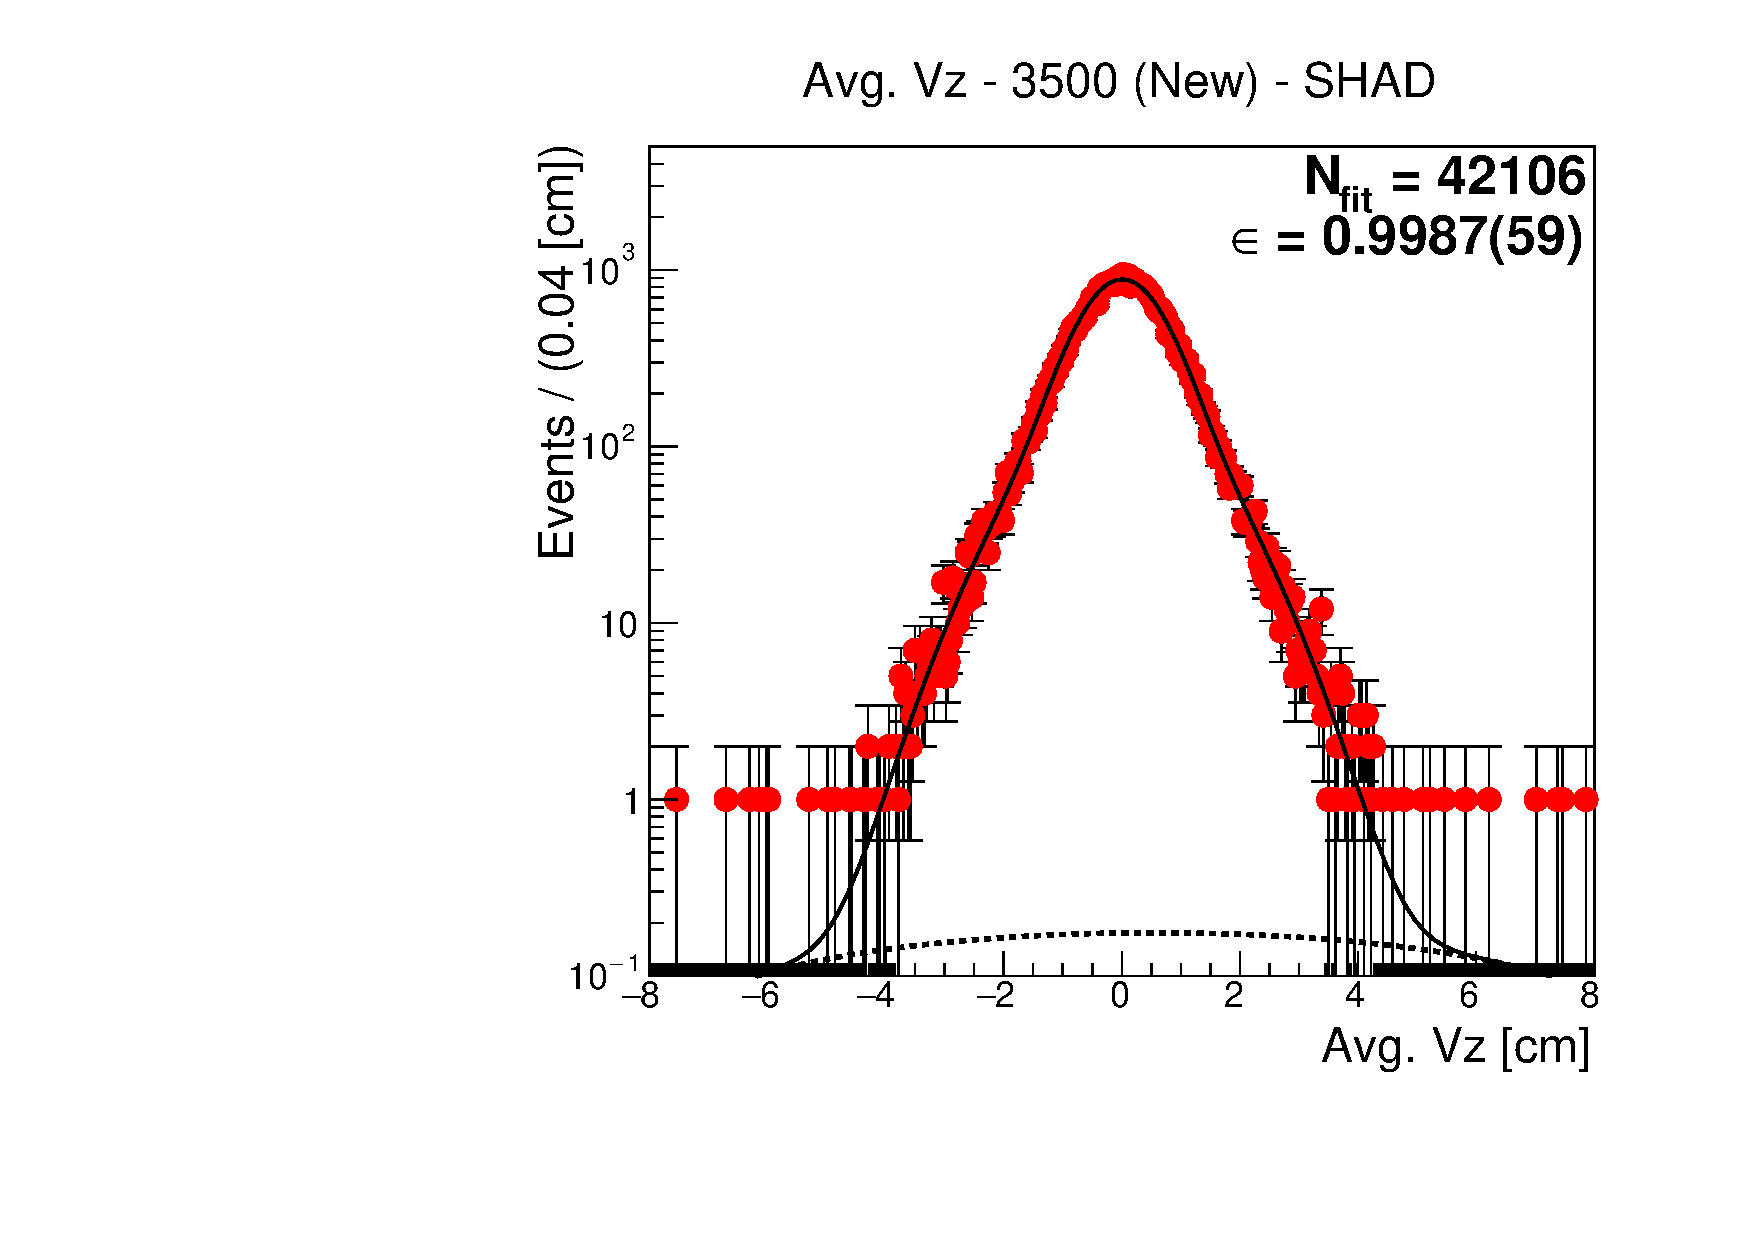
\includegraphics[scale=0.25]{figures/plots/nonDDbar_fit_results/3650_new/fit_new_3500_data_SHAD.pdf}
\hspace{-0.5cm}
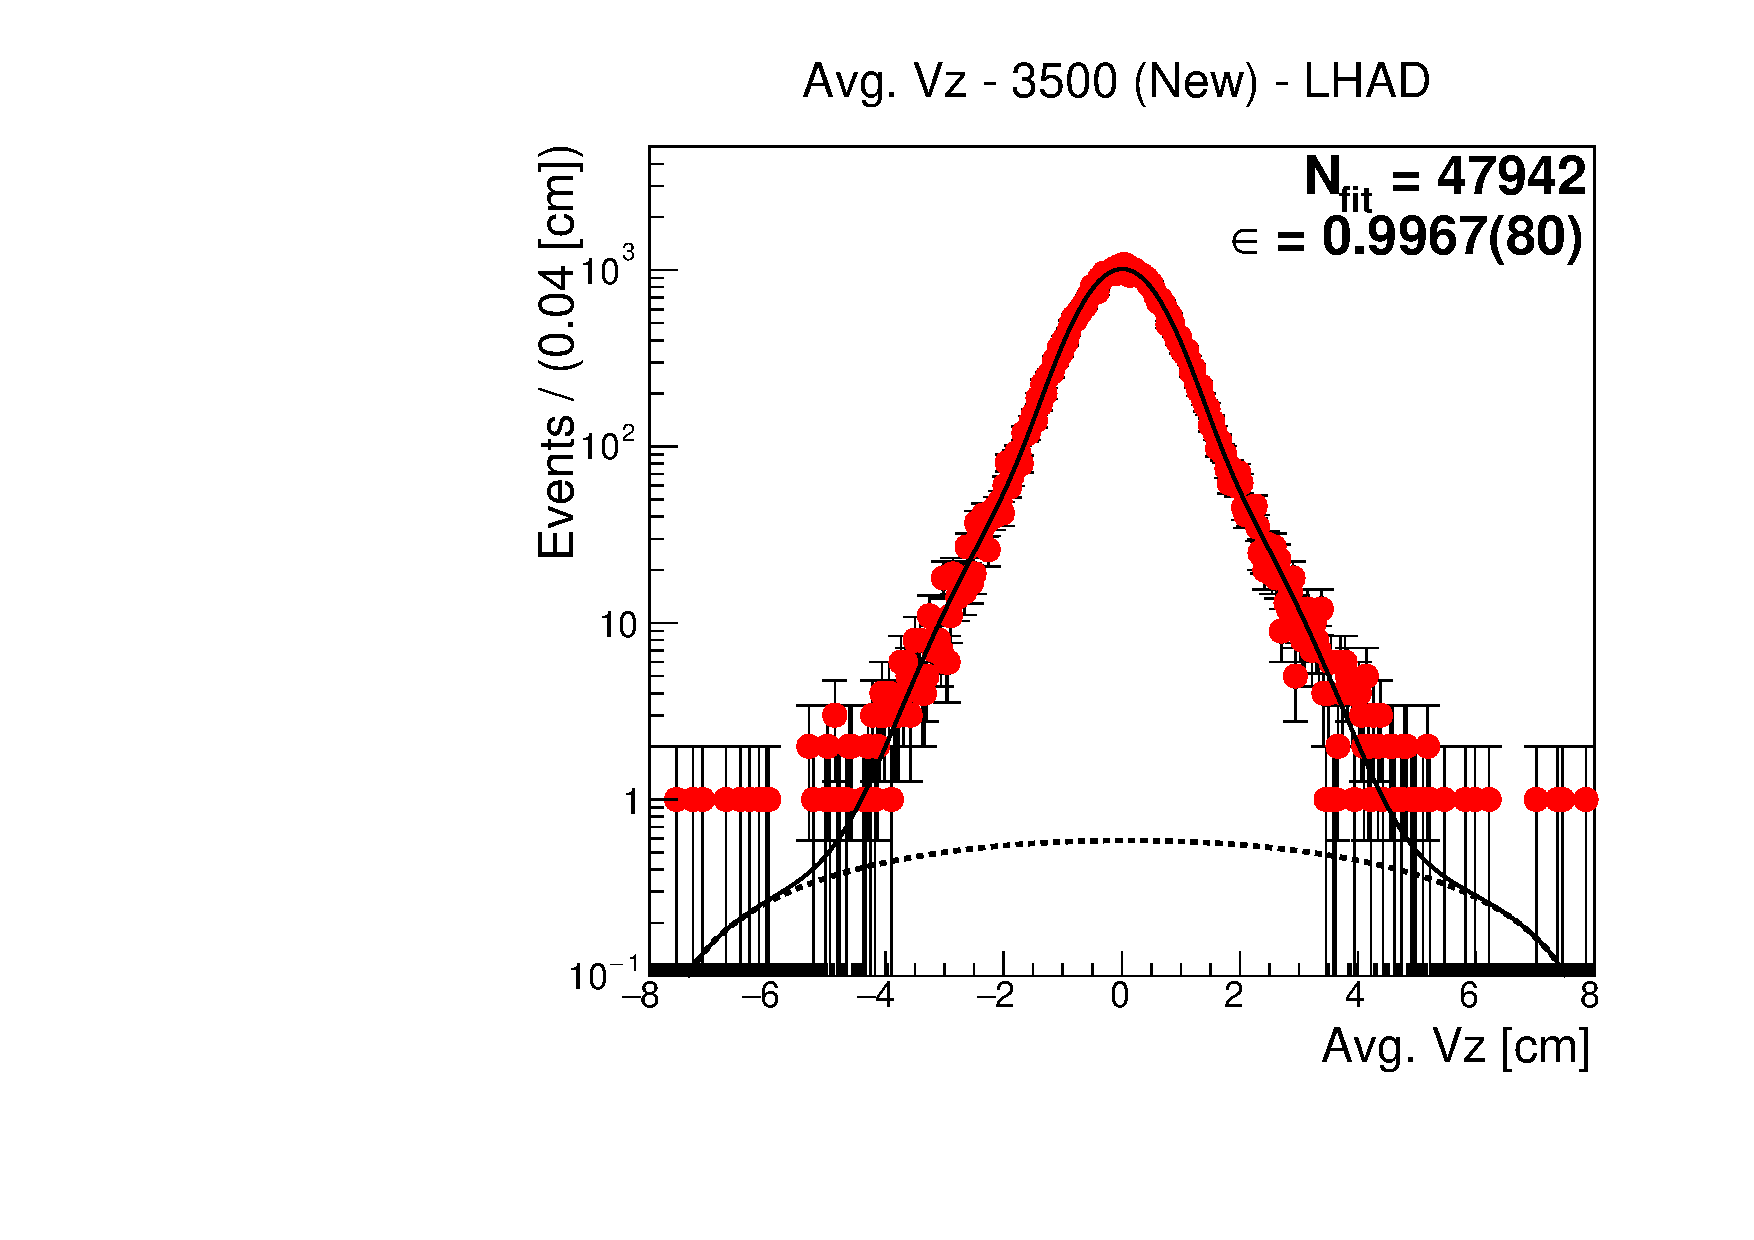
\includegraphics[scale=0.25]{figures/plots/nonDDbar_fit_results/3650_new/fit_new_3500_data_LHAD.pdf}
\hspace{-0.5cm}
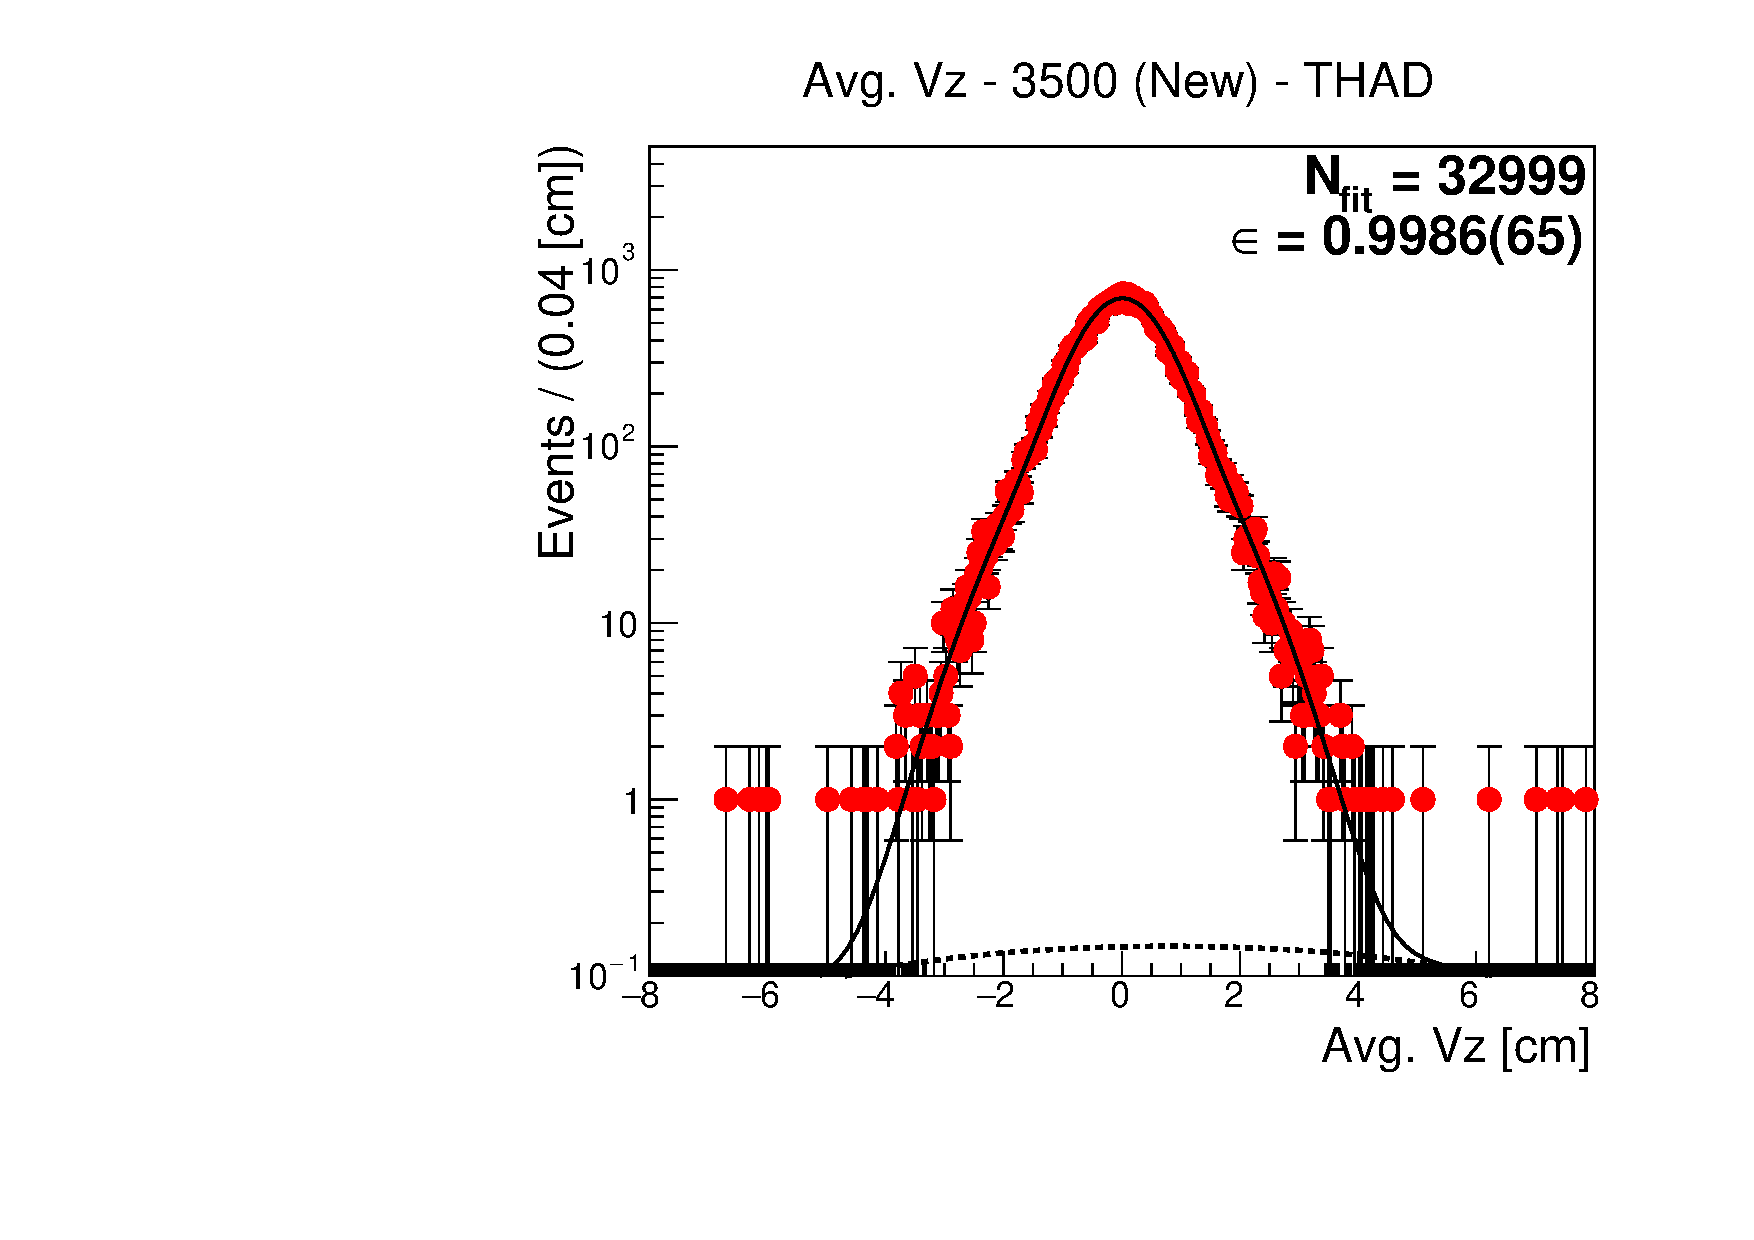
\includegraphics[scale=0.25]{figures/plots/nonDDbar_fit_results/3650_new/fit_new_3500_data_THAD.pdf}
\caption{The number of hadrons found in the 3500 (New) data sample.}
{This includes results for SHAD (left), LHAD (middle), and THAD (right).}
\label{fig:hadron_fits_3500_new}
\end{figure}


\begin{figure}[H]
\centering
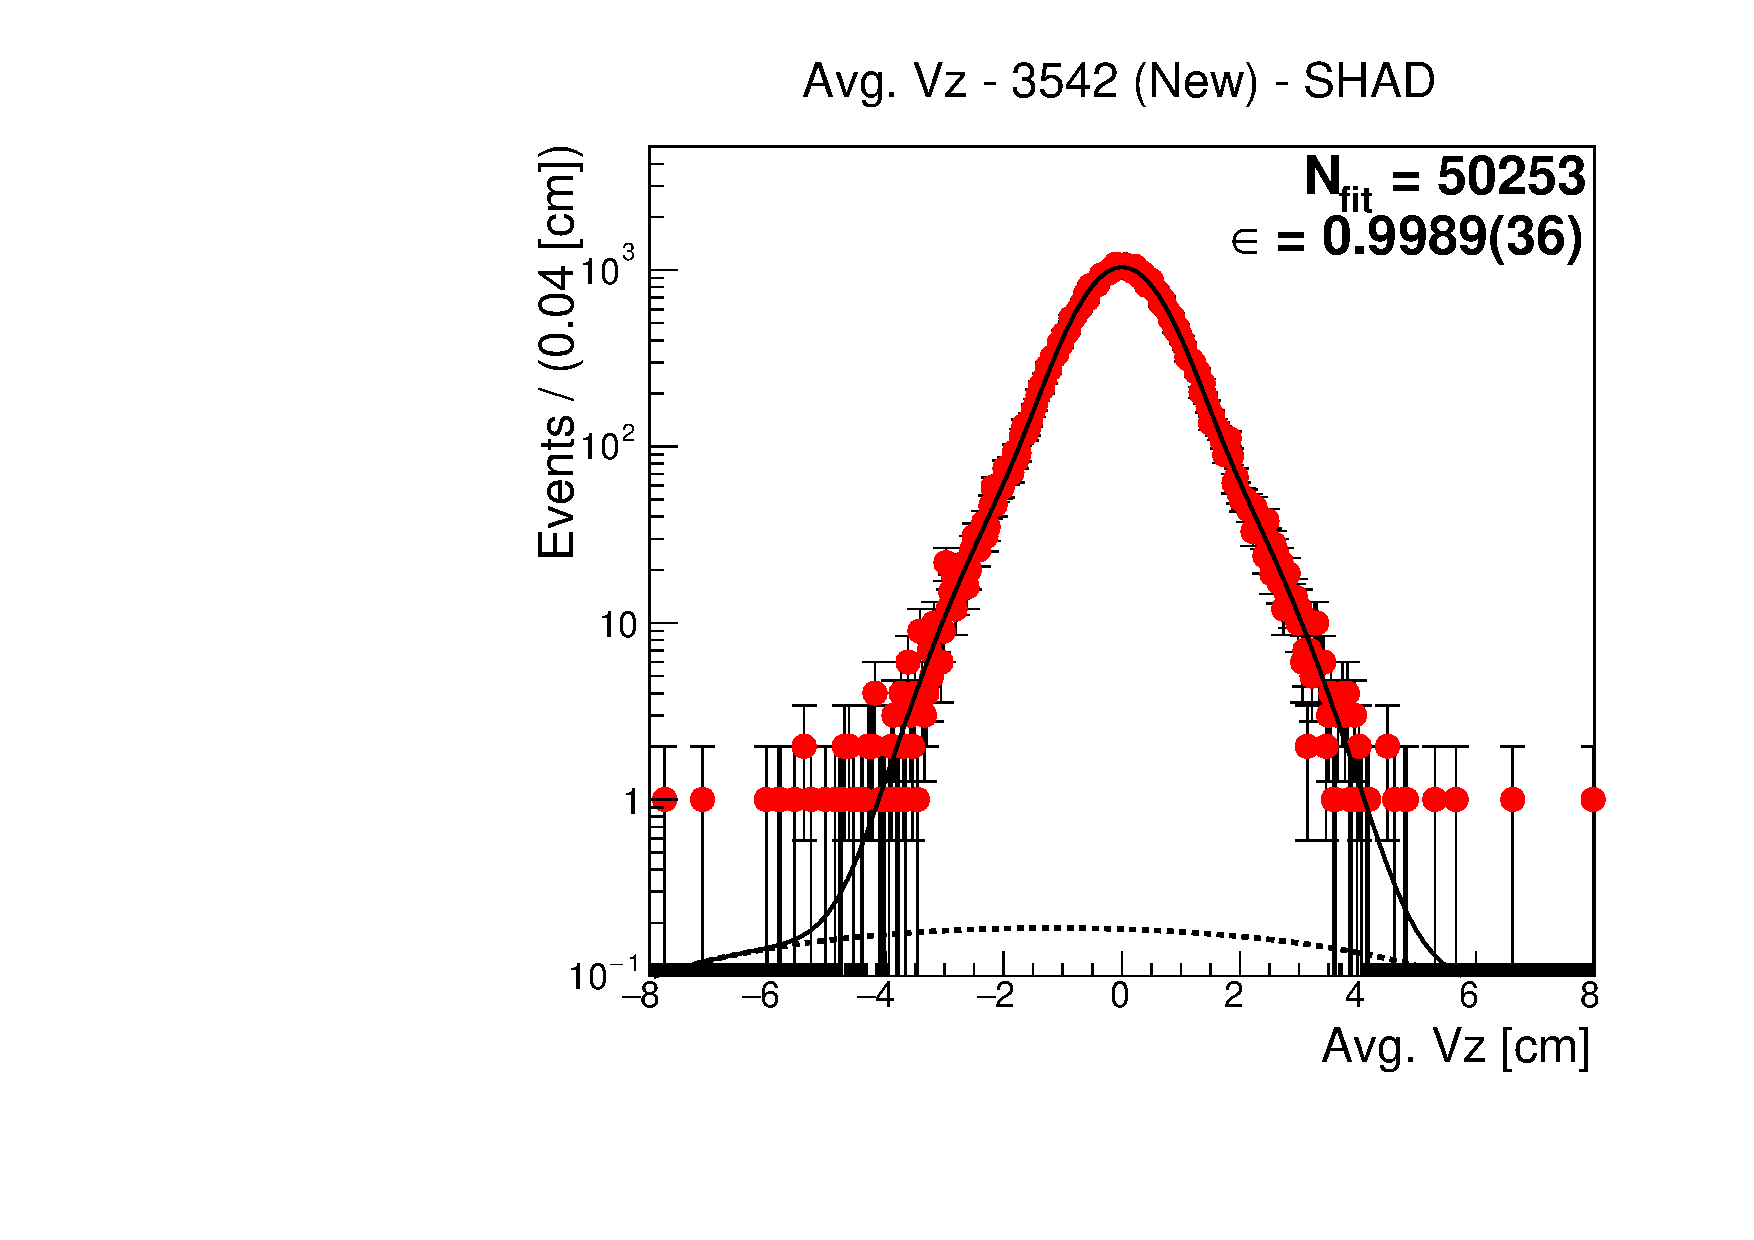
\includegraphics[scale=0.25]{figures/plots/nonDDbar_fit_results/3650_new/fit_new_3542_data_SHAD.pdf}
\hspace{-0.5cm}
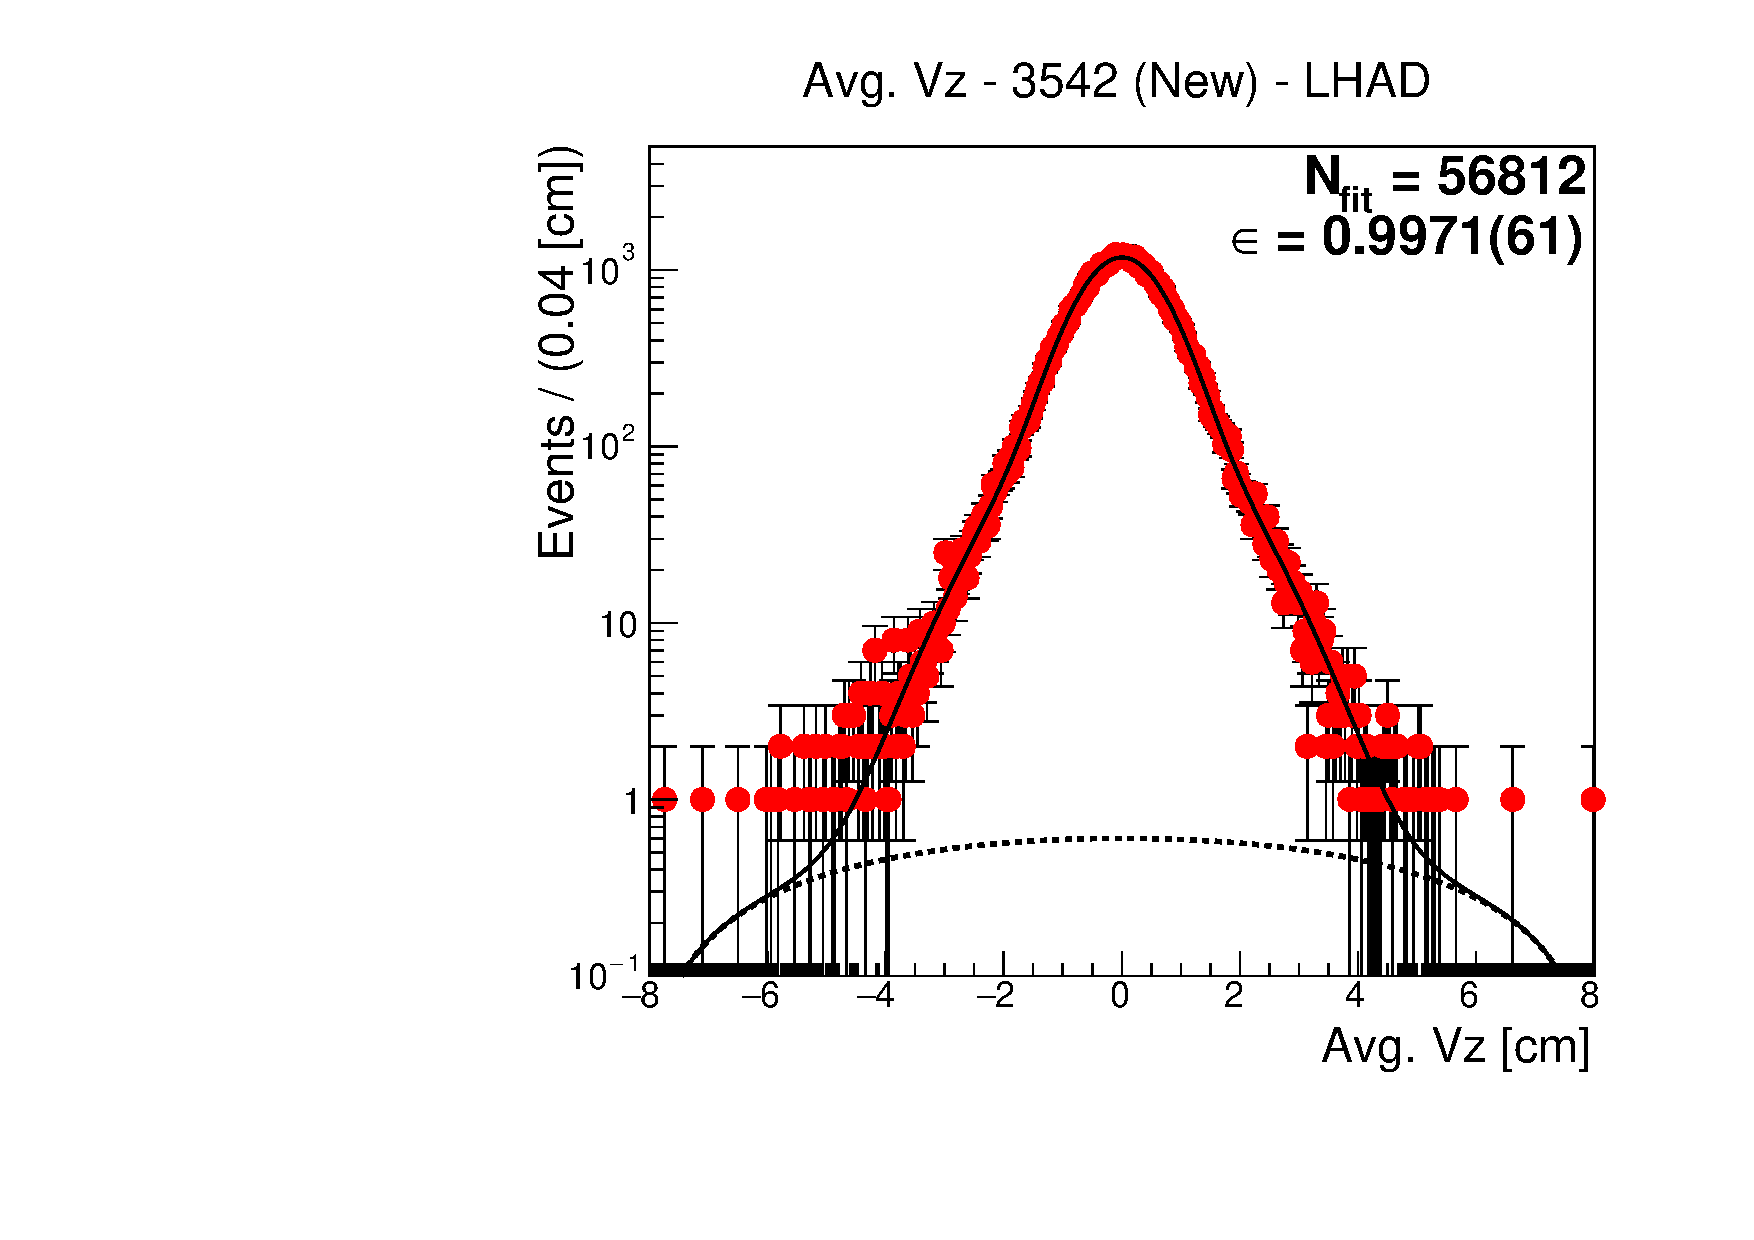
\includegraphics[scale=0.25]{figures/plots/nonDDbar_fit_results/3650_new/fit_new_3542_data_LHAD.pdf}
\hspace{-0.5cm}
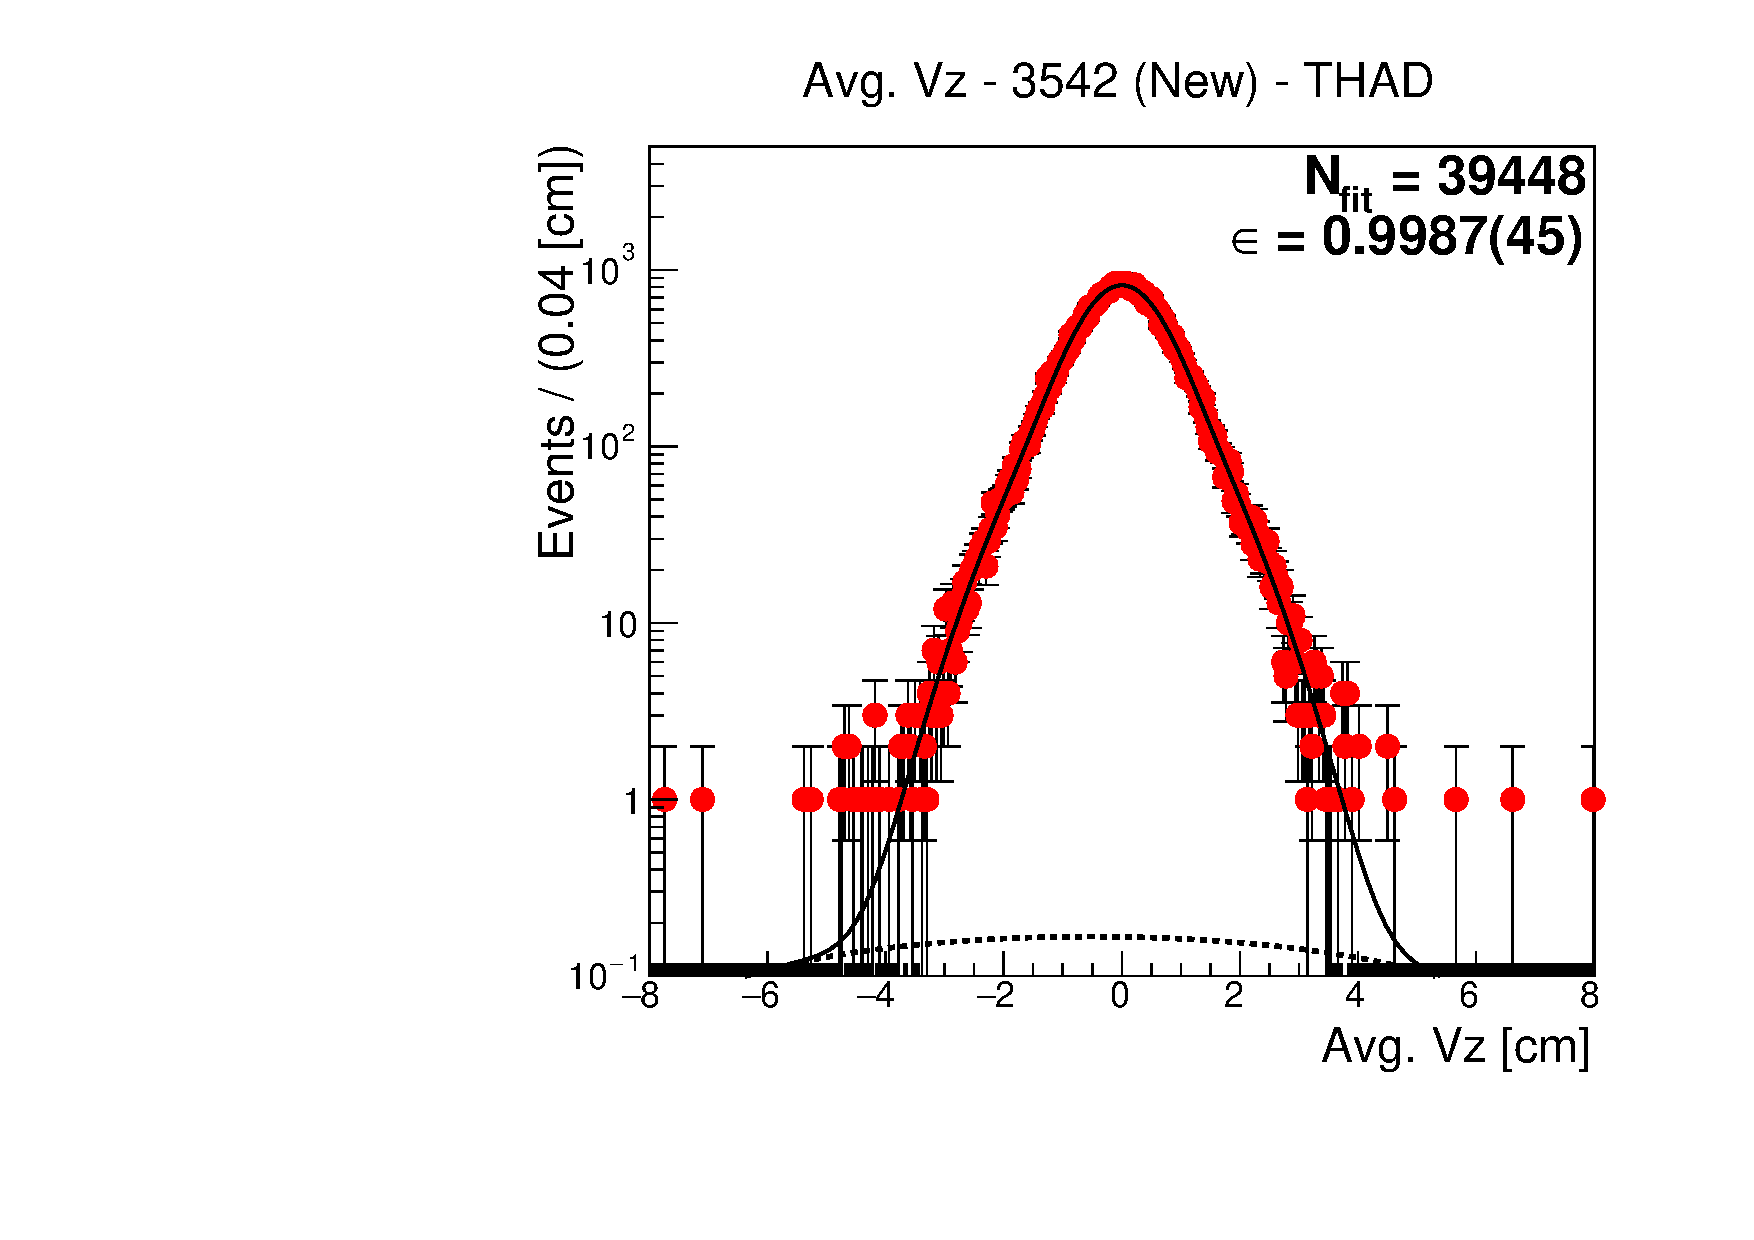
\includegraphics[scale=0.25]{figures/plots/nonDDbar_fit_results/3650_new/fit_new_3542_data_THAD.pdf}
\caption{The number of hadrons found in the 3542 (New) data sample.}
{This includes results for SHAD (left), LHAD (middle), and THAD (right).}
\label{fig:hadron_fits_3542_new}
\end{figure}


\begin{figure}[H]
\centering
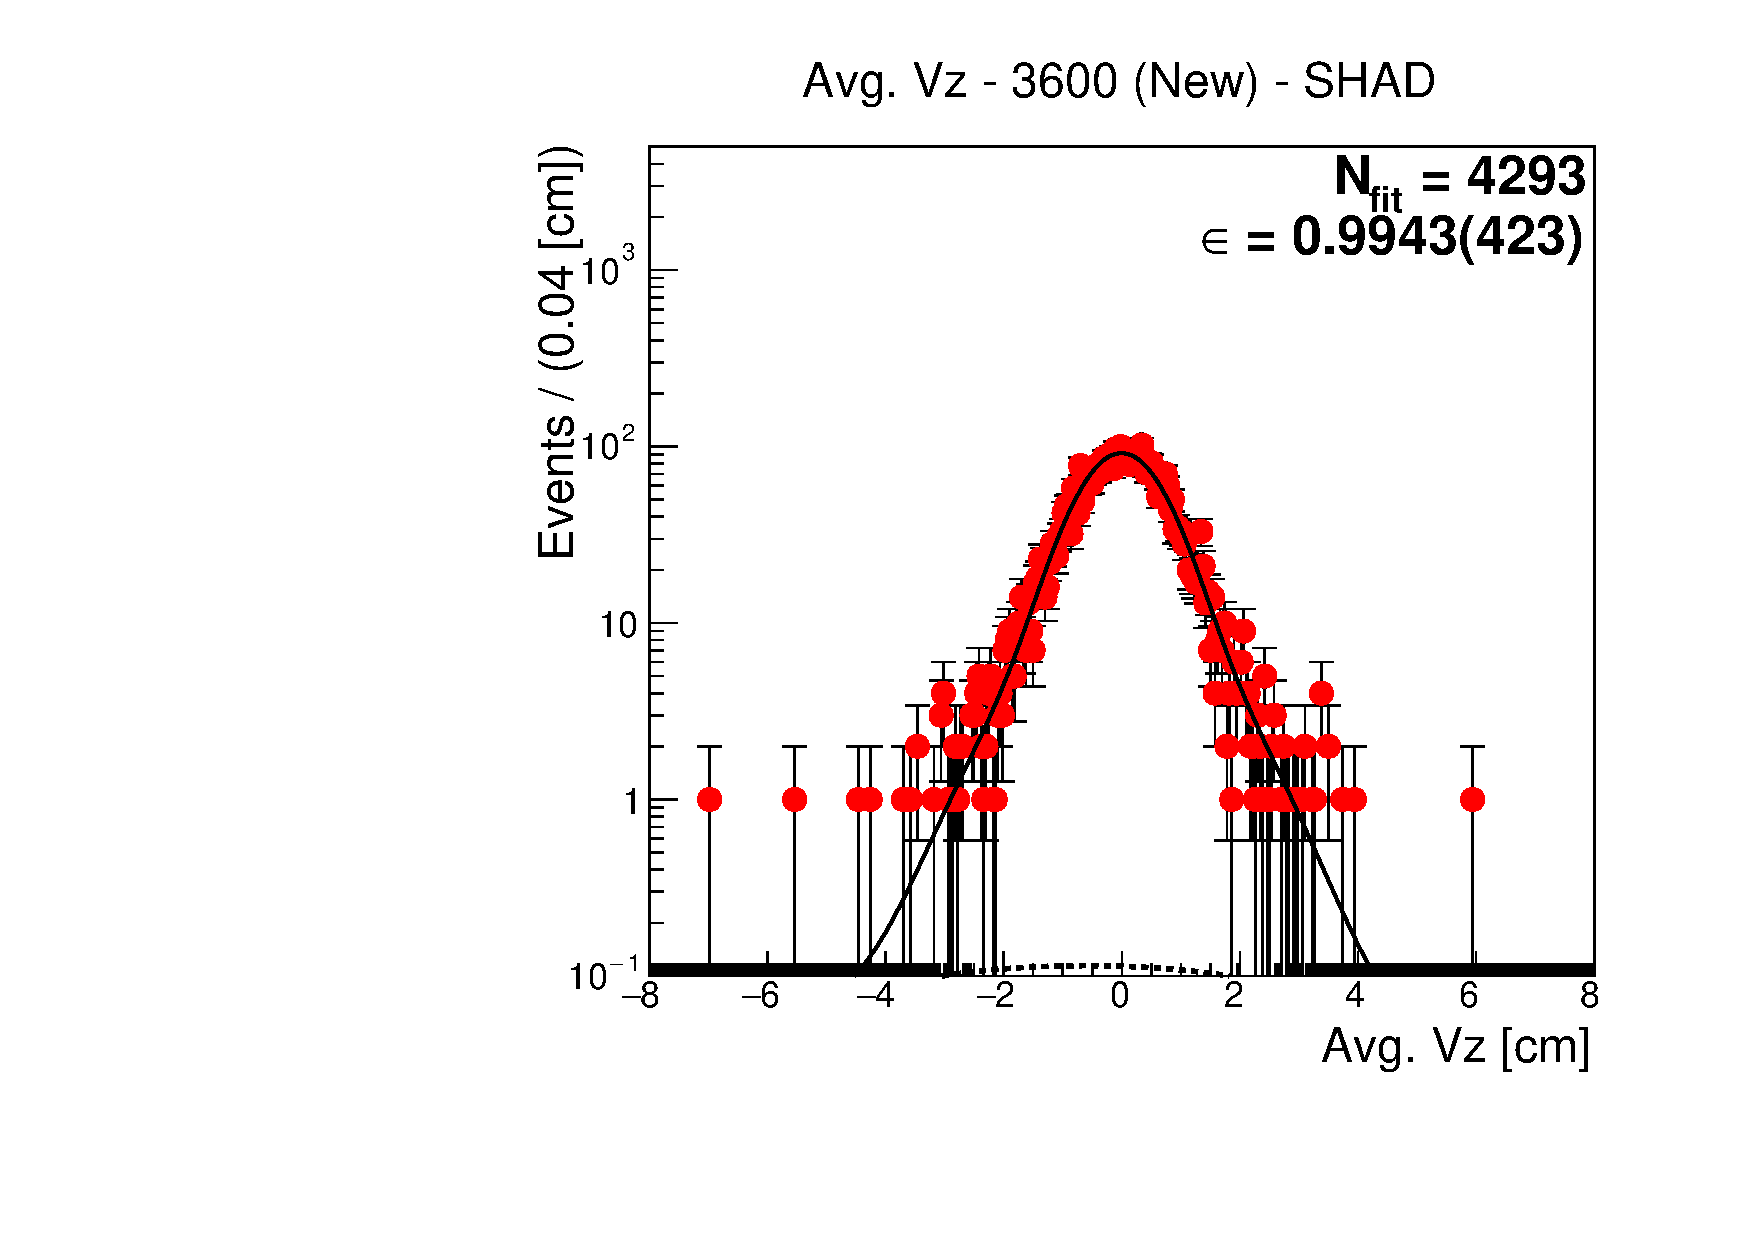
\includegraphics[scale=0.25]{figures/plots/nonDDbar_fit_results/3650_new/fit_new_3600_data_SHAD.pdf}
\hspace{-0.5cm}
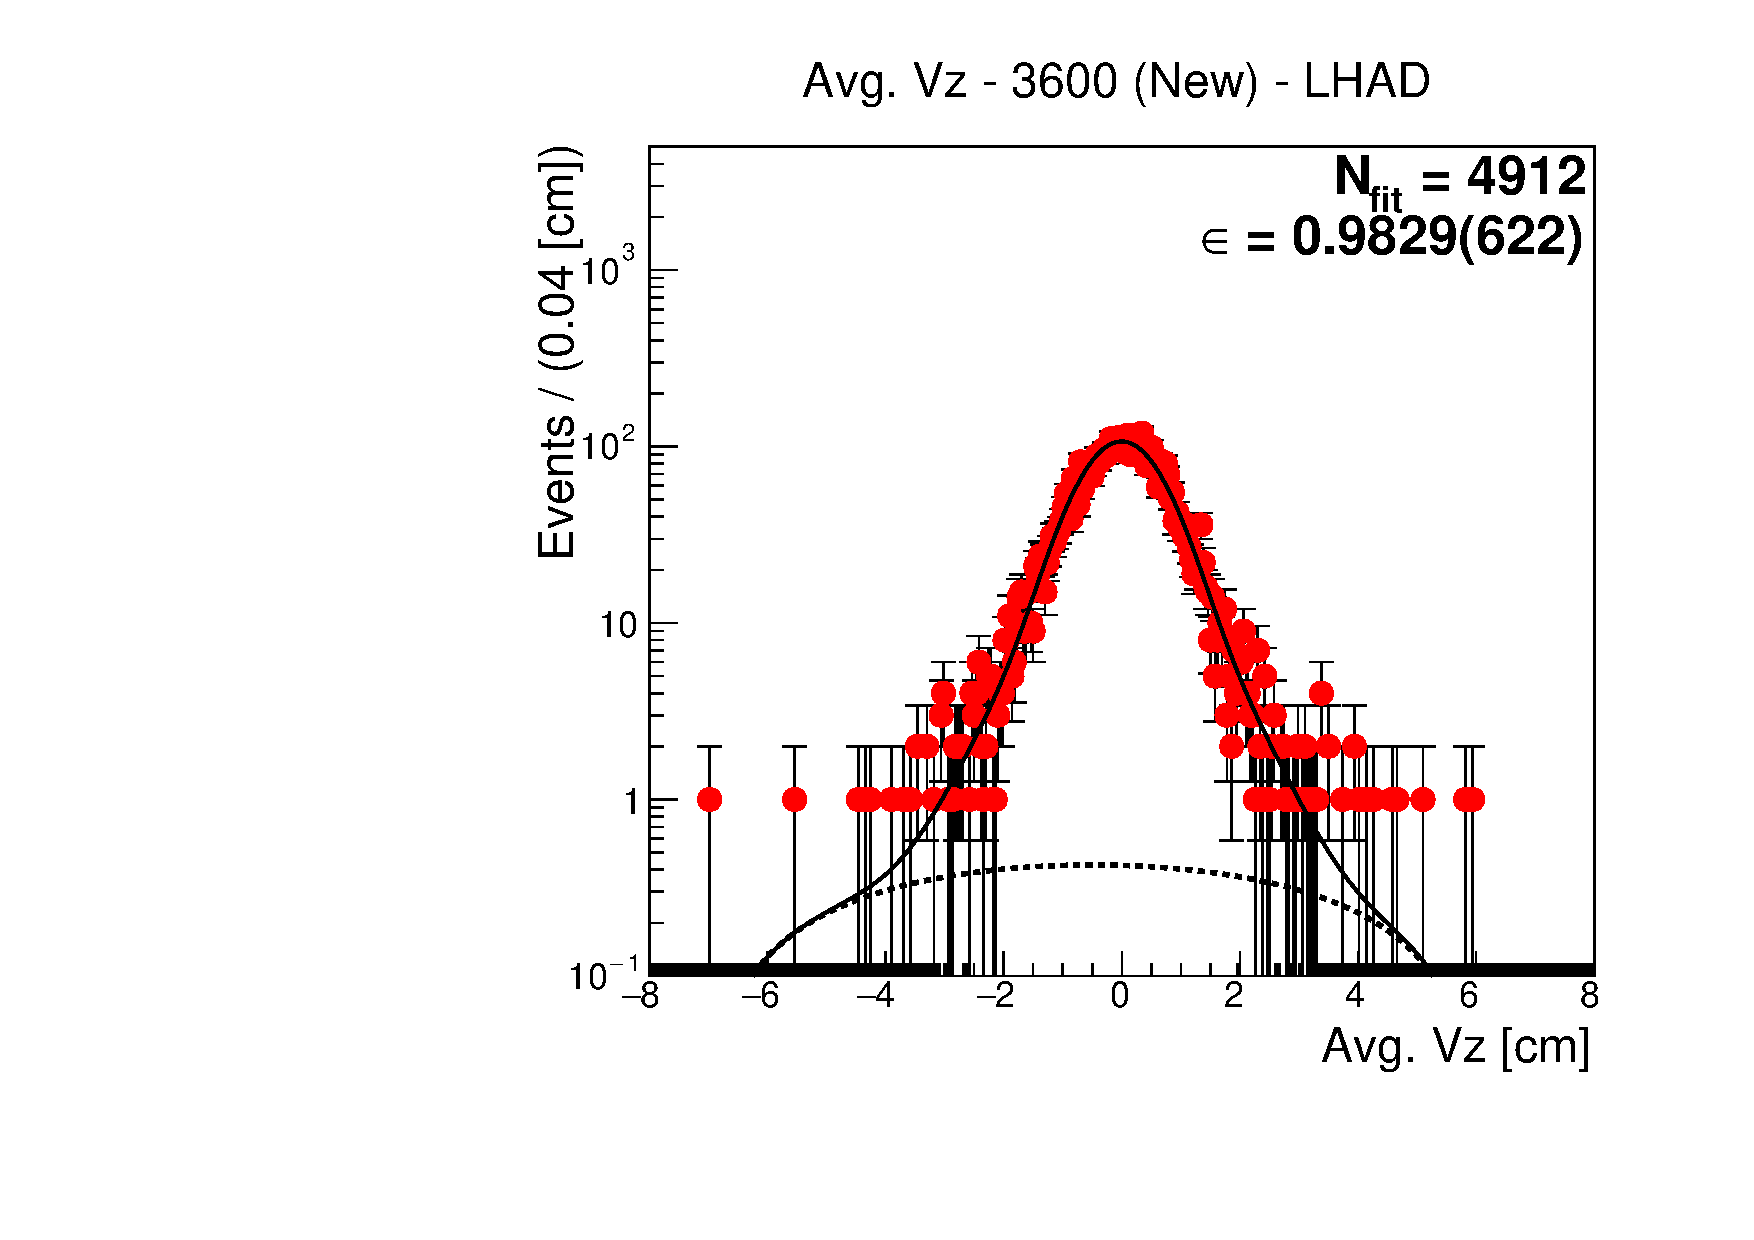
\includegraphics[scale=0.25]{figures/plots/nonDDbar_fit_results/3650_new/fit_new_3600_data_LHAD.pdf}
\hspace{-0.5cm}
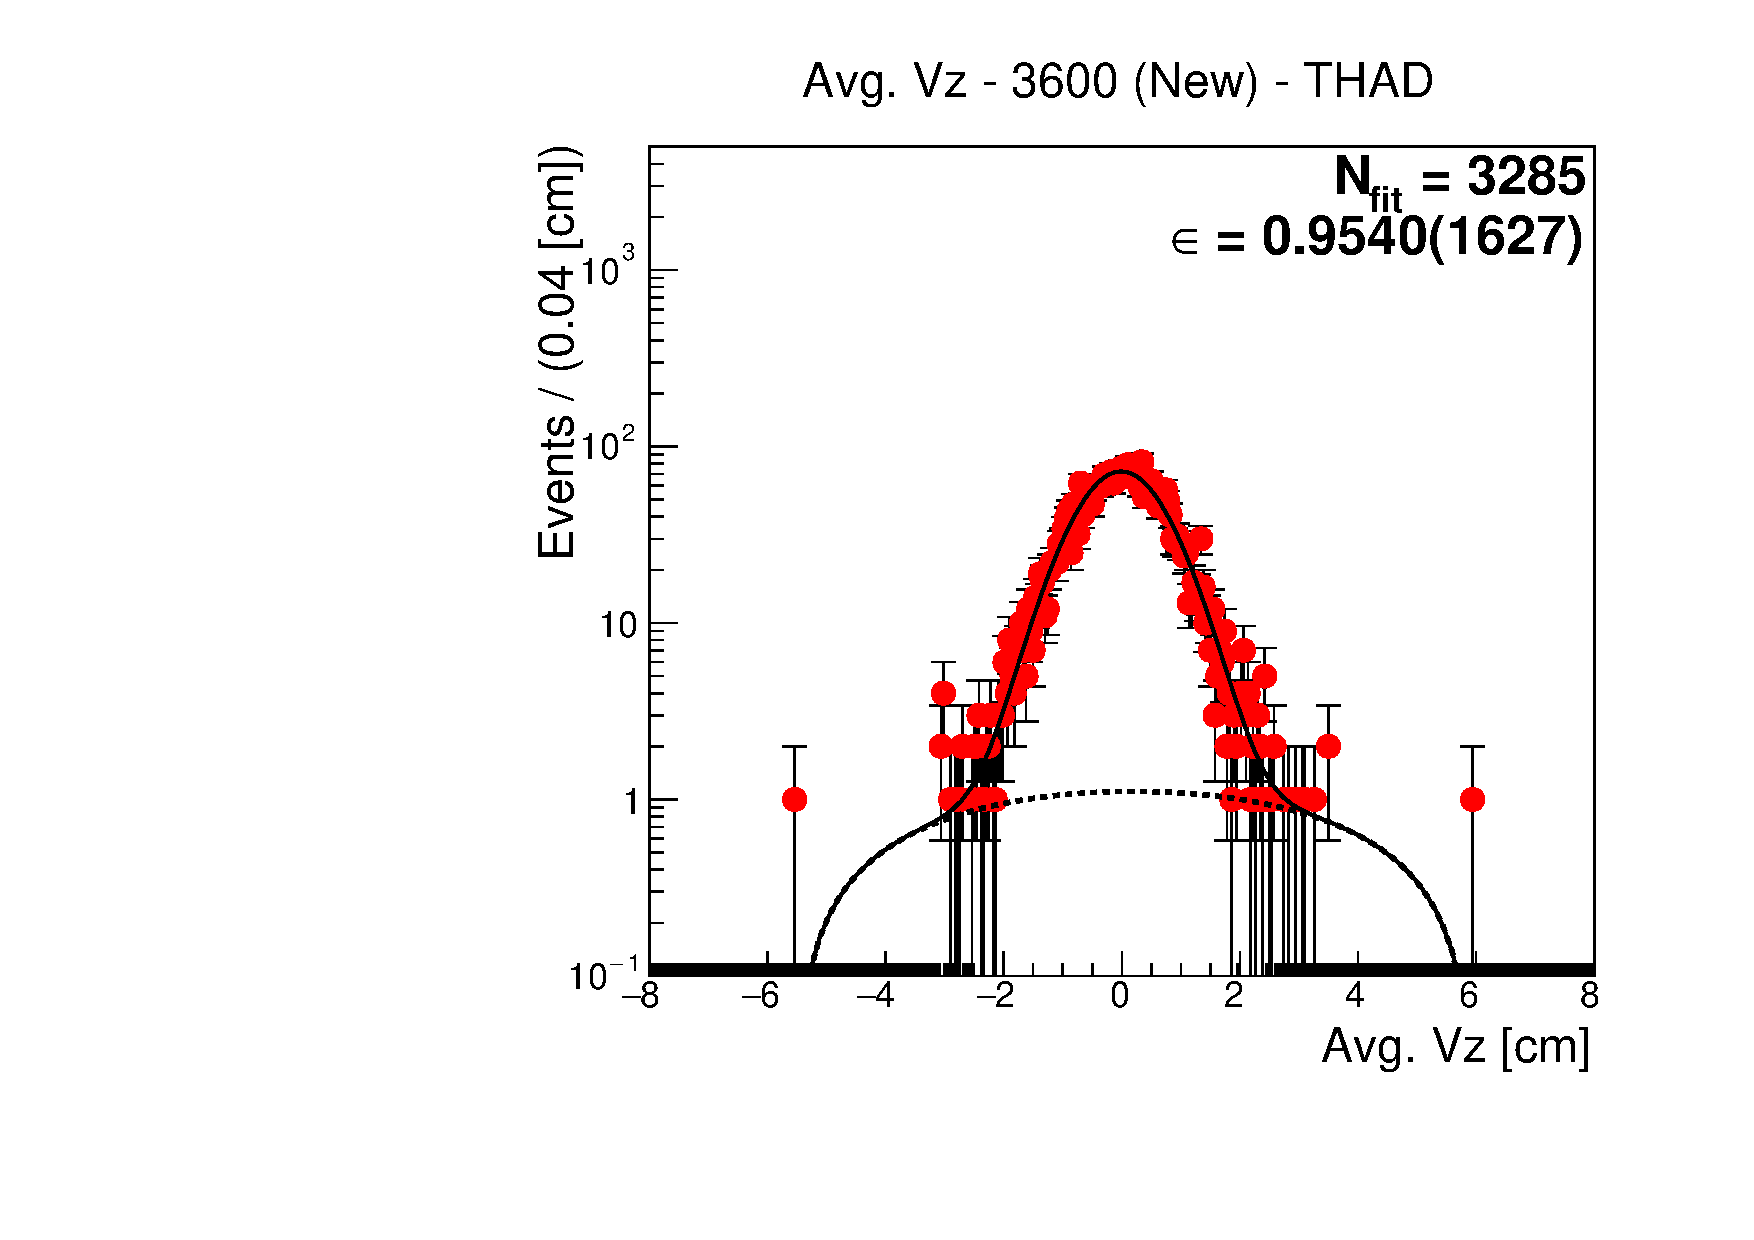
\includegraphics[scale=0.25]{figures/plots/nonDDbar_fit_results/3650_new/fit_new_3600_data_THAD.pdf}
\caption{The number of hadrons found in the 3600 (New) data sample.}
{This includes results for SHAD (left), LHAD (middle), and THAD (right).}
\label{fig:hadron_fits_3600_new}
\end{figure}


\begin{figure}[H]
\centering
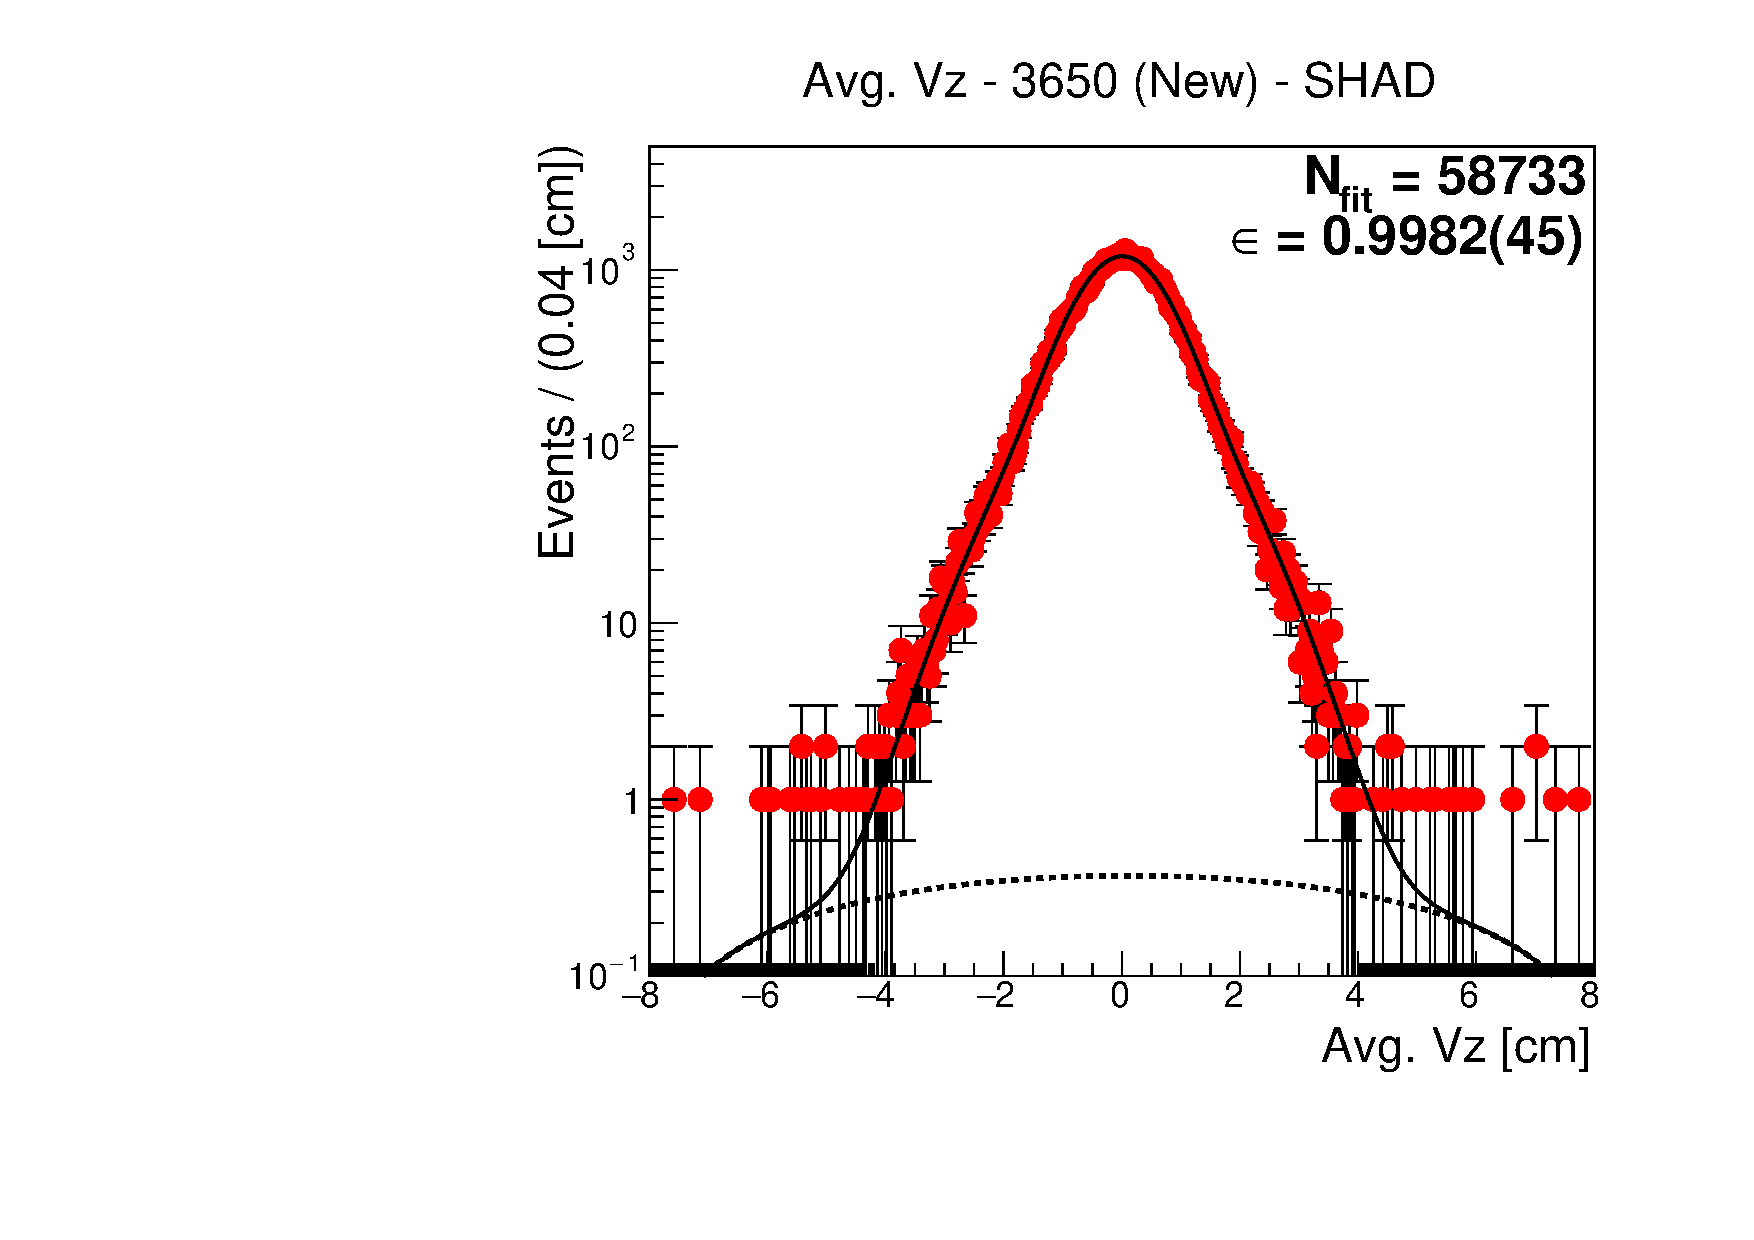
\includegraphics[scale=0.25]{figures/plots/nonDDbar_fit_results/3650_new/fit_new_3650_data_SHAD.pdf}
\hspace{-0.5cm}
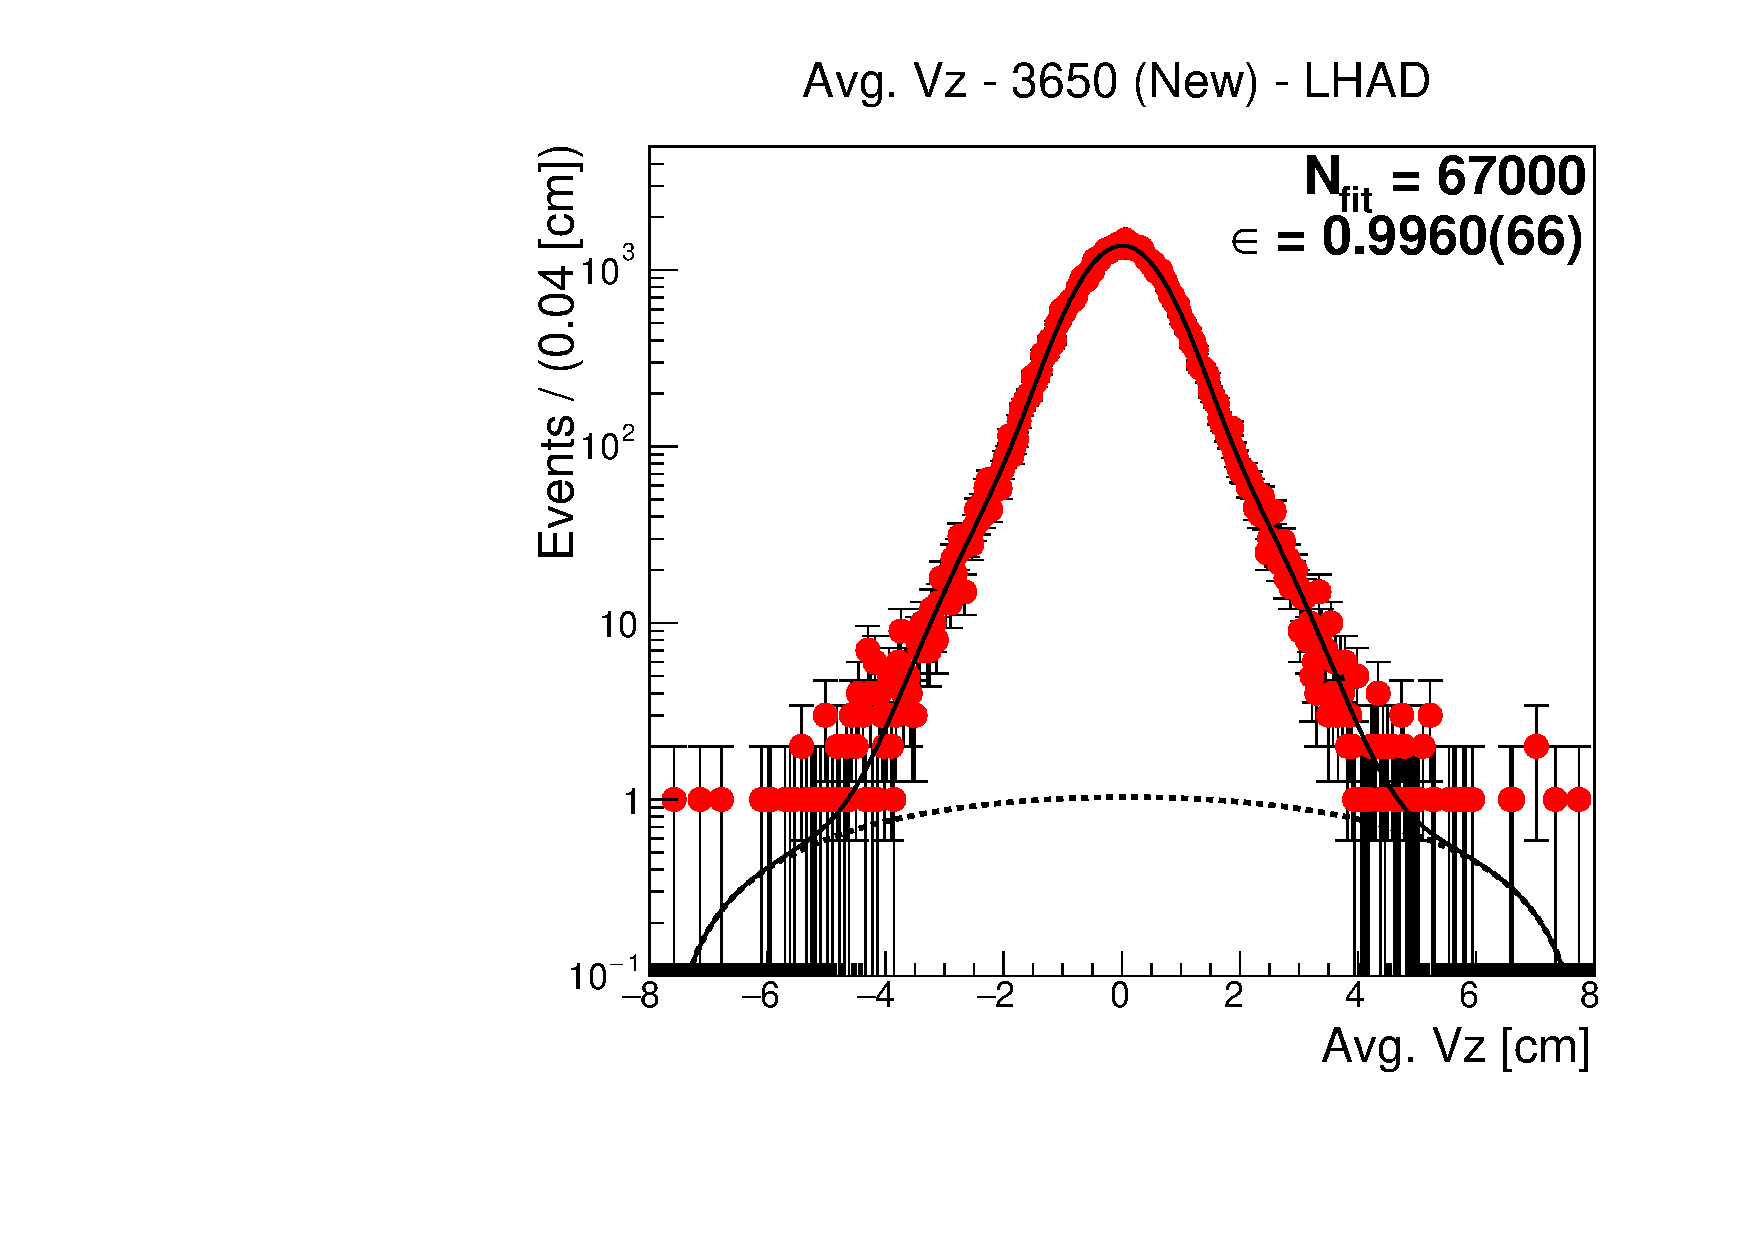
\includegraphics[scale=0.25]{figures/plots/nonDDbar_fit_results/3650_new/fit_new_3650_data_LHAD.pdf}
\hspace{-0.5cm}
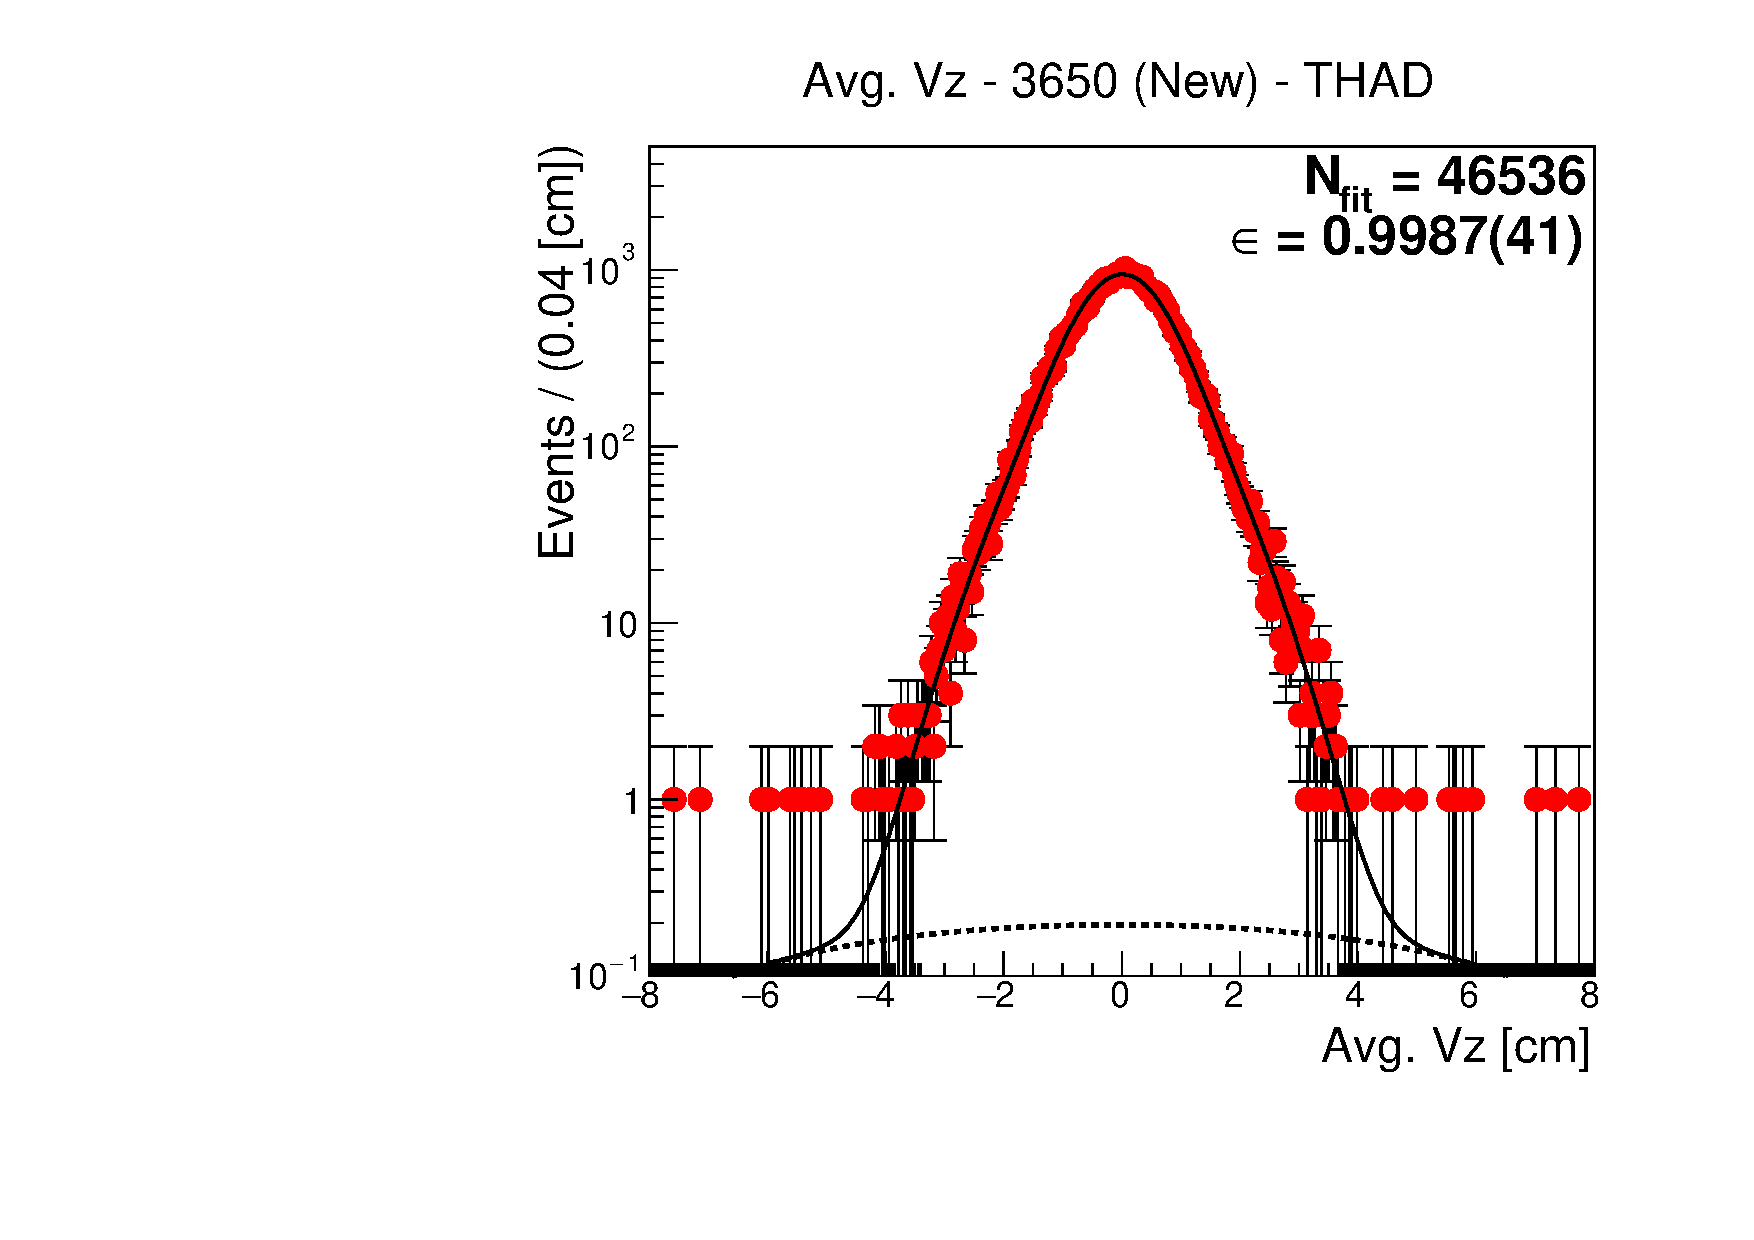
\includegraphics[scale=0.25]{figures/plots/nonDDbar_fit_results/3650_new/fit_new_3650_data_THAD.pdf}
\caption{The number of hadrons found in the 3650 (New) data sample.}
{This includes results for SHAD (left), LHAD (middle), and THAD (right).}
\label{fig:hadron_fits_3650_new}
\end{figure}


\begin{figure}[H]
\centering
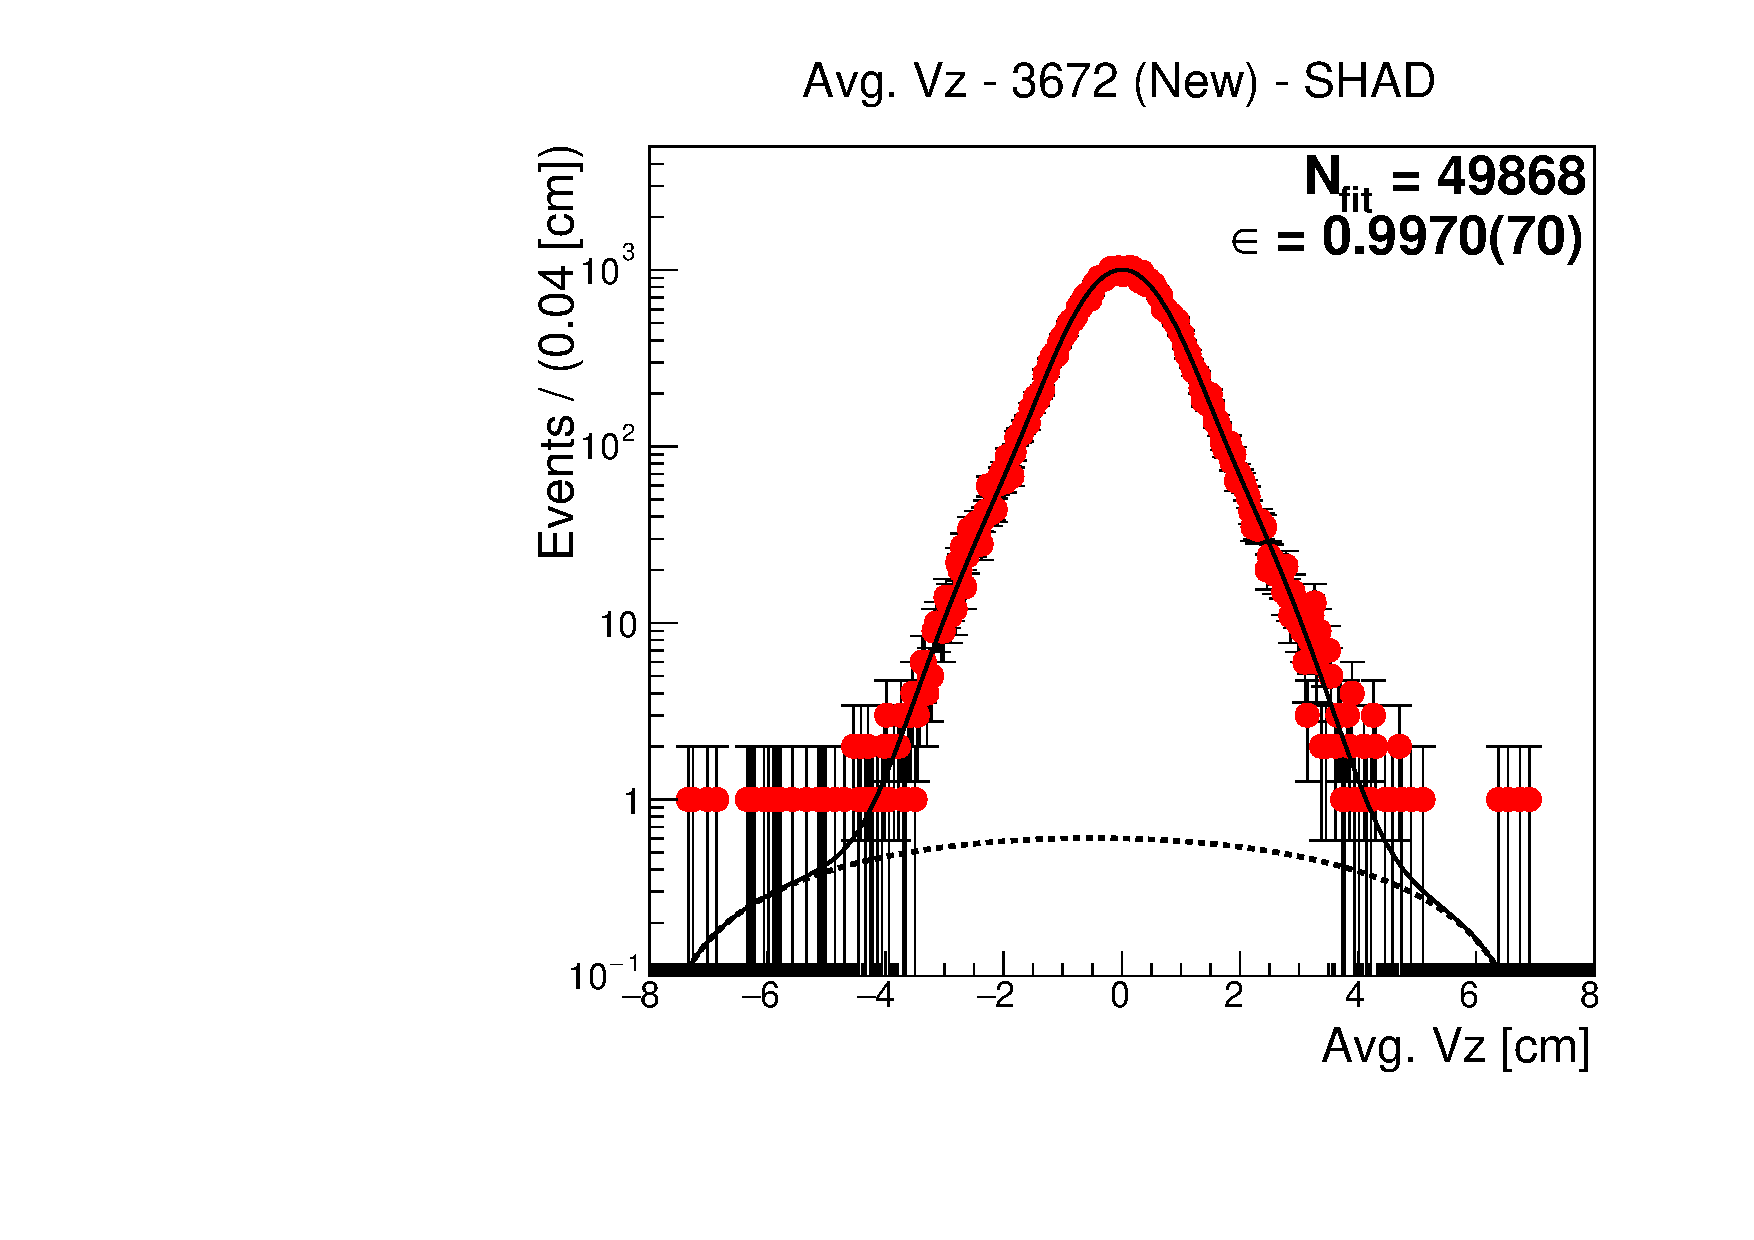
\includegraphics[scale=0.25]{figures/plots/nonDDbar_fit_results/3650_new/fit_new_3671_data_SHAD.pdf}
\hspace{-0.5cm}
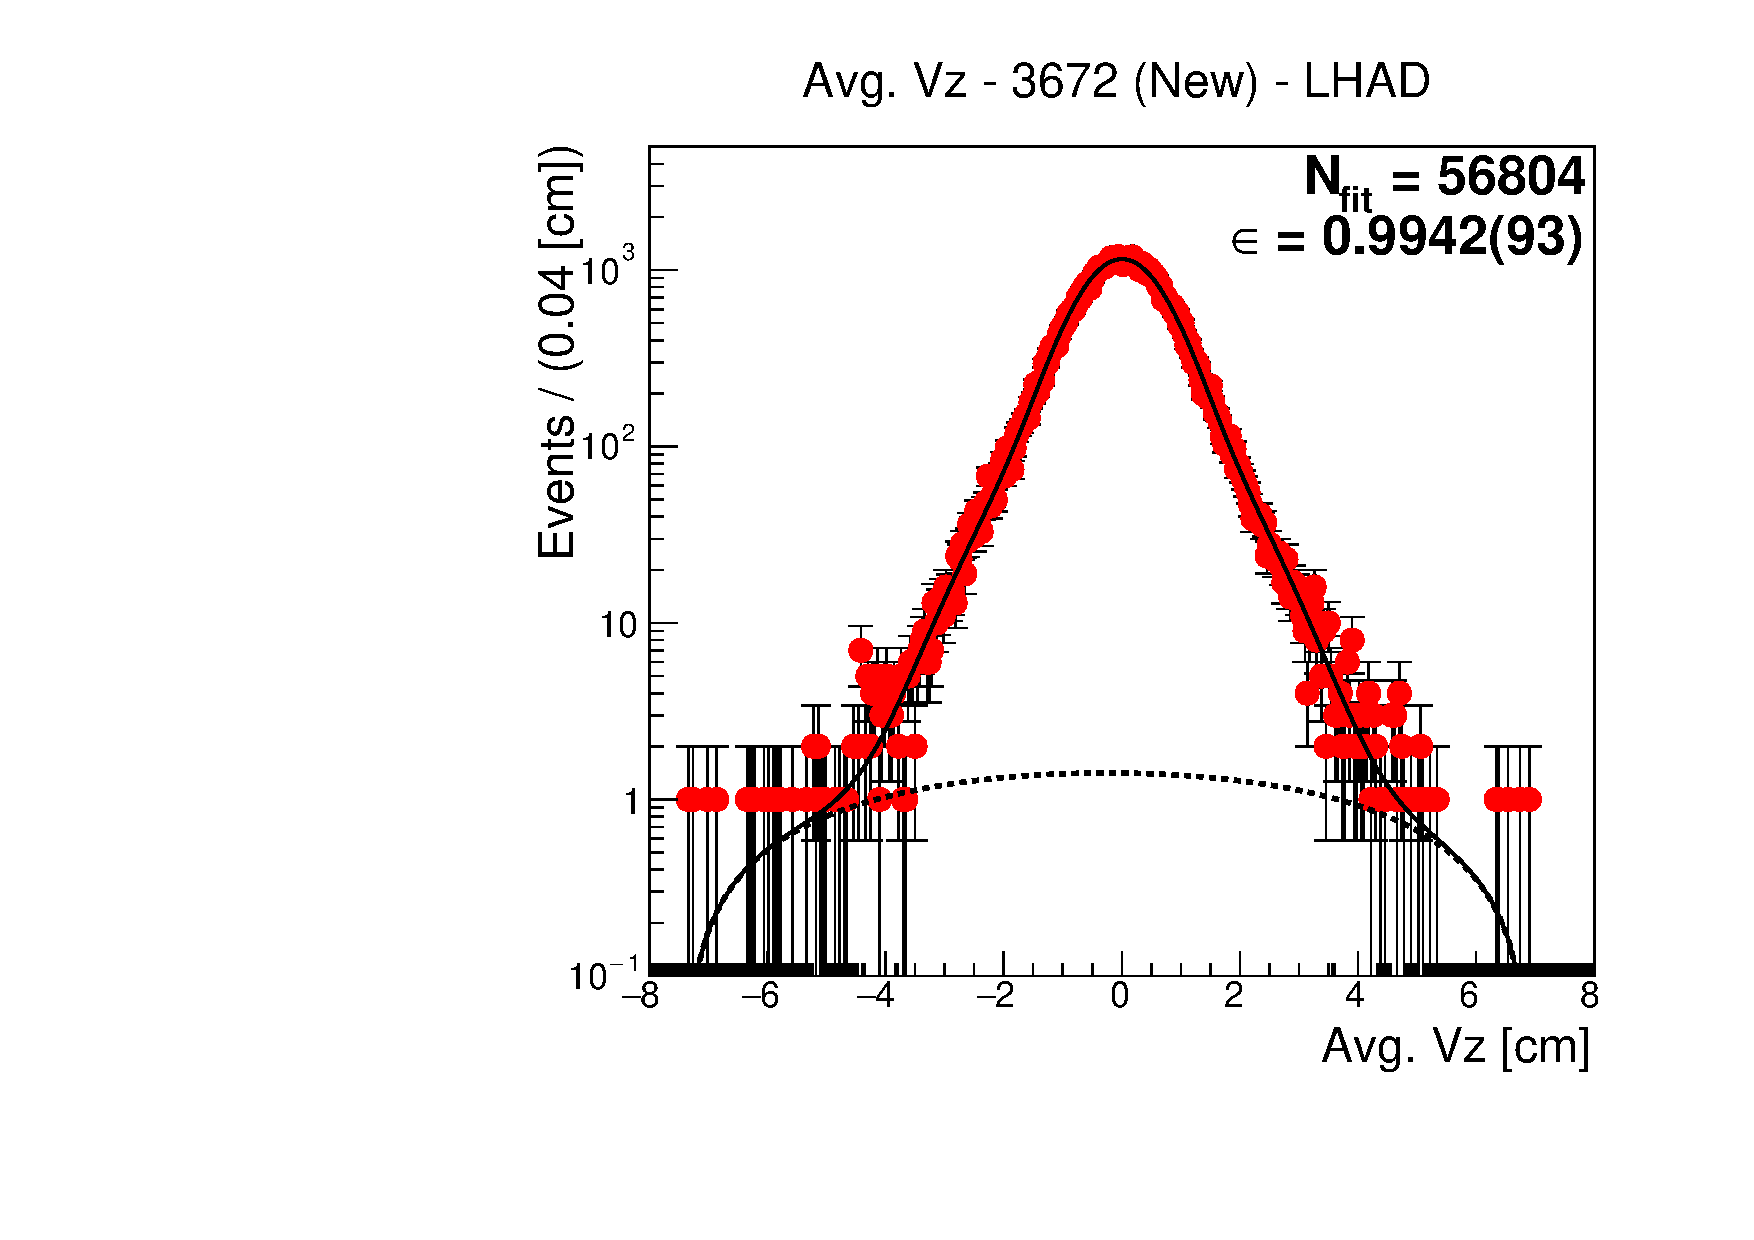
\includegraphics[scale=0.25]{figures/plots/nonDDbar_fit_results/3650_new/fit_new_3671_data_LHAD.pdf}
\hspace{-0.5cm}
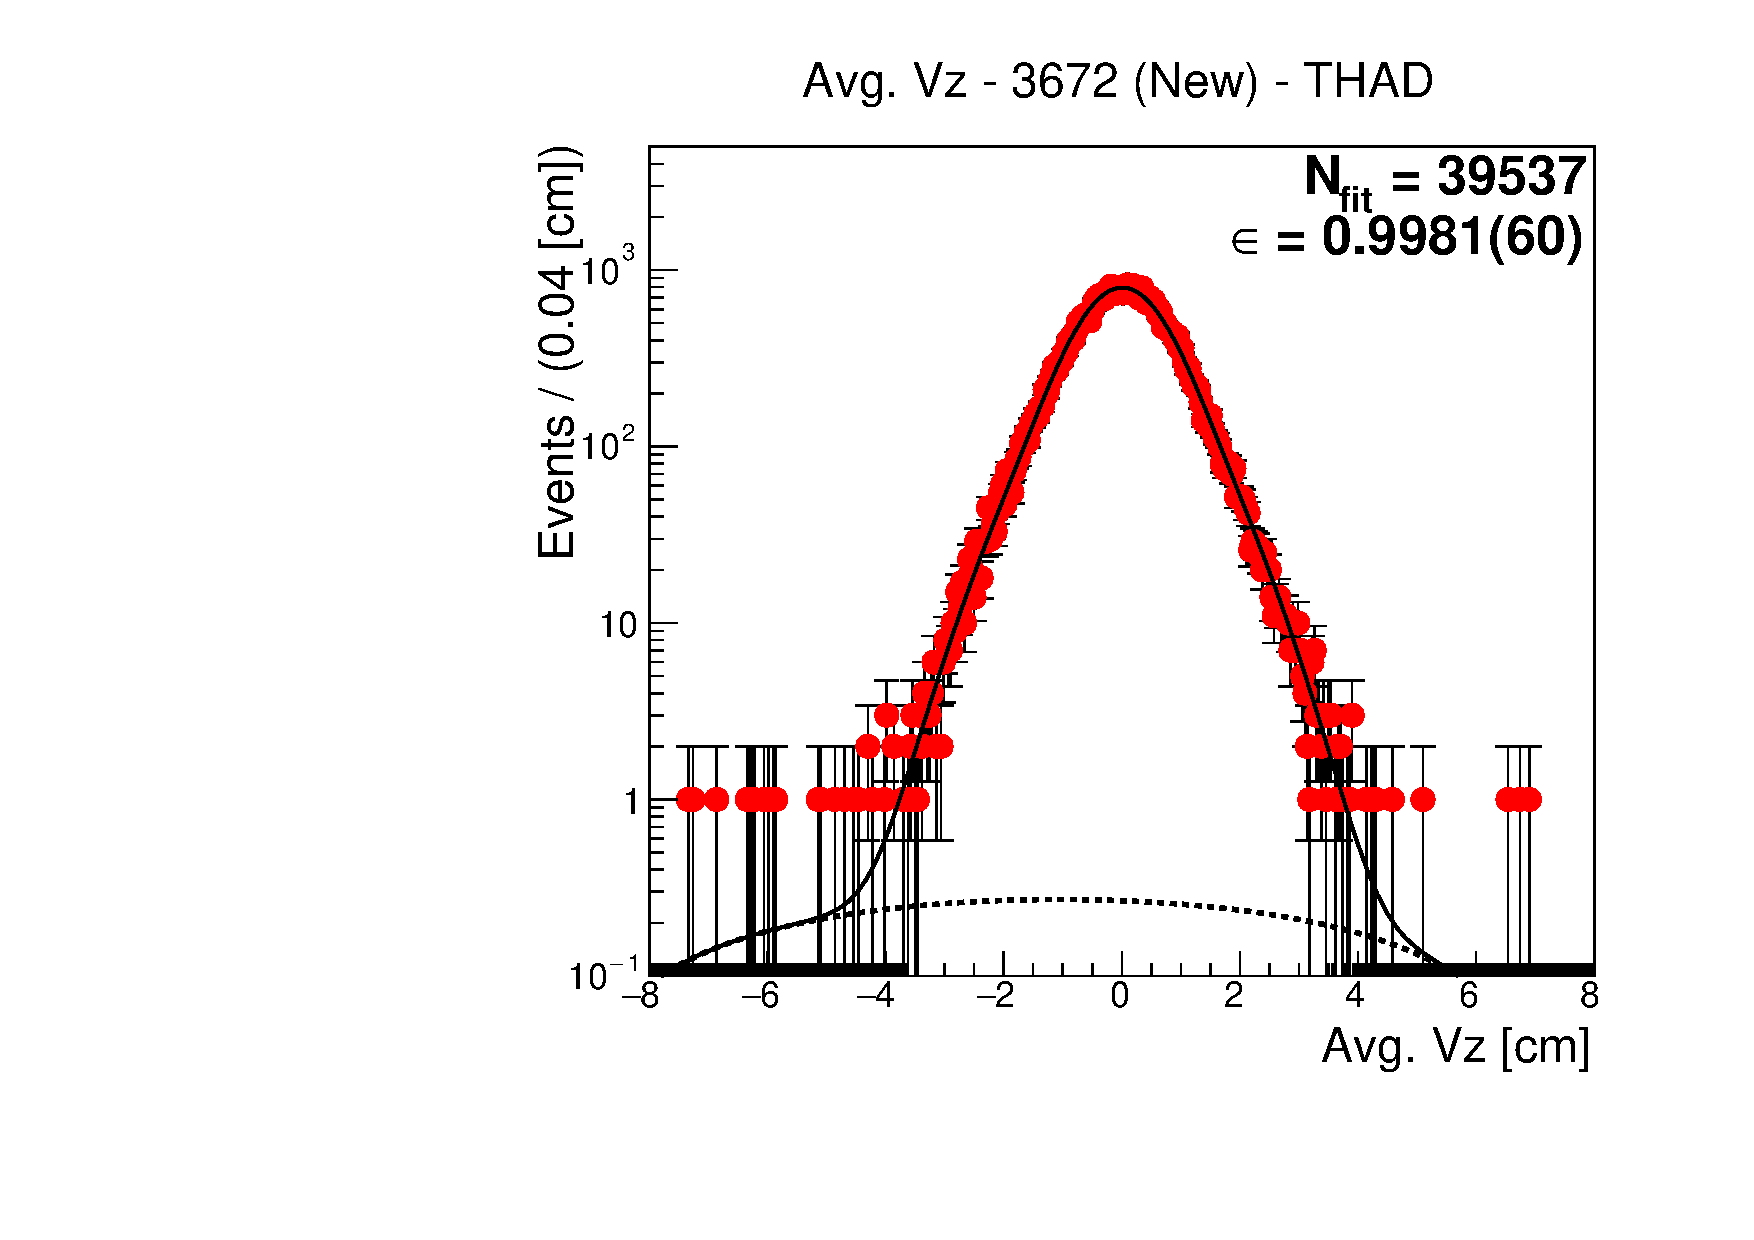
\includegraphics[scale=0.25]{figures/plots/nonDDbar_fit_results/3650_new/fit_new_3671_data_THAD.pdf}
\caption{The number of hadrons found in the 3671 (New) data sample.}
{This includes results for SHAD (left), LHAD (middle), and THAD (right).}
\label{fig:hadron_fits_3671_new}
\end{figure}



\begin{table}[H]
\centering
\renewcommand\arraystretch{1.0}

\begin{tabular}{c|r|cr@{$\; \pm \;$}rc cr@{$\; \pm \;$}rc cr@{$\; \pm \;$}rc}
\hline
\multicolumn{14}{c}{3500 (New) Reconstruction} \\
\hline
Sample & $\sigma$ [\si{\pb}] & \multicolumn{4}{c}{$\effmc$ (SHAD) [\%]} & \multicolumn{4}{c}{$\effmc$ (LHAD) [\%]} & \multicolumn{4}{c}{$\effmc$ (THAD) [\%]} \\
\hline
$\tautau$       & 0.000 && \mcd{2}         &&& \mcd{2}         &&& \mcd{2}         & \\
$\yjpsi$        & 1.831 &&  47.079 & 0.077 &&&  56.117 & 0.084 &&&  35.320 & 0.066 & \\
$\twophoton$    & 1.240 &&   2.380 & 0.017 &&&   4.924 & 0.025 &&&   1.644 & 0.014 & \\
$\psip^\dagger$ & 0.006 &&  62.989 & 0.008 &&&  69.288 & 0.008 &&&  51.694 & 0.007 & \\
\hline          
\end{tabular}

\vspace{0.5cm}

\begin{tabular}{c|r|cr@{$\; \pm \;$}rc cr@{$\; \pm \;$}rc cr@{$\; \pm \;$}rc}
\hline
\multicolumn{14}{c}{3542 (New) Reconstruction} \\
\hline
Sample & $\sigma$ [\si{\pb}] & \multicolumn{4}{c}{$\effmc$ (SHAD) [\%]} & \multicolumn{4}{c}{$\effmc$ (LHAD) [\%]} & \multicolumn{4}{c}{$\effmc$ (THAD) [\%]} \\
\hline
$\tautau$       & 0.000 && \mcd{2}        &&& \mcd{2}        &&& \mcd{2}        & \\
$\yjpsi$        & 1.632 && 47.188 & 0.072 &&& 56.430 & 0.079 &&& 35.355 & 0.063 & \\
$\twophoton$    & 1.270 &&  2.386 & 0.016 &&&  5.046 & 0.024 &&&  1.633 & 0.013 & \\
$\psip^\dagger$ & 0.009 && 62.989 & 0.008 &&& 69.288 & 0.008 &&& 51.694 & 0.007 & \\
\hline          
\end{tabular}

\vspace{0.5cm}

\begin{tabular}{c|r|cr@{$\; \pm \;$}rc cr@{$\; \pm \;$}rc cr@{$\; \pm \;$}rc}
\hline
\multicolumn{14}{c}{3600 (New) Reconstruction} \\
\hline
Sample & $\sigma$ [\si{\pb}] & \multicolumn{4}{c}{$\effmc$ (SHAD) [\%]} & \multicolumn{4}{c}{$\effmc$ (LHAD) [\%]} & \multicolumn{4}{c}{$\effmc$ (THAD) [\%]} \\
\hline
$\tautau$       & 1.262 && 12.851 & 0.080 &&& 29.096 & 0.121 &&& 10.040 & 0.071 & \\
$\yjpsi$        & 1.412 && 47.524 & 0.154 &&& 56.902 & 0.169 &&& 35.703 & 0.134 & \\
$\twophoton$    & 1.311 &&  2.651 & 0.036 &&&  5.089 & 0.050 &&&  1.897 & 0.031 & \\
$\psip^\dagger$ & 0.024 && 62.989 & 0.008 &&& 69.288 & 0.008 &&& 51.694 & 0.007 & \\
\hline          
\end{tabular}

\vspace{0.5cm}

\begin{tabular}{c|r|cr@{$\; \pm \;$}rc cr@{$\; \pm \;$}rc cr@{$\; \pm \;$}rc}
\hline
\multicolumn{14}{c}{3650 (New) Reconstruction} \\
\hline
Sample & $\sigma$ [\si{\pb}] & \multicolumn{4}{c}{$\effmc$ (SHAD) [\%]} & \multicolumn{4}{c}{$\effmc$ (LHAD) [\%]} & \multicolumn{4}{c}{$\effmc$ (THAD) [\%]} \\
\hline
$\tautau$       & 1.844 && 12.964 & 0.033 &&& 28.939 & 0.049 &&& 10.154 & 0.029 & \\
$\yjpsi$        & 1.260 && 47.414 & 0.063 &&& 57.043 & 0.069 &&& 35.701 & 0.055 & \\
$\twophoton$    & 1.346 &&  2.410 & 0.014 &&&  4.675 & 0.020 &&&  1.682 & 0.012 & \\
$\psip^\dagger$ & 0.110 && 62.989 & 0.008 &&& 69.288 & 0.008 &&& 51.694 & 0.007 & \\
\hline          
\end{tabular}

\vspace{0.5cm}

\begin{tabular}{c|r|cr@{$\; \pm \;$}rc cr@{$\; \pm \;$}rc cr@{$\; \pm \;$}rc}
\hline
\multicolumn{14}{c}{3671 (New) Reconstruction} \\
\hline
Sample & $\sigma$ [\si{\pb}] & \multicolumn{4}{c}{$\effmc$ (SHAD) [\%]} & \multicolumn{4}{c}{$\effmc$ (LHAD) [\%]} & \multicolumn{4}{c}{$\effmc$ (THAD) [\%]} \\
\hline
$\tautau$       & 2.026 && 12.997 & 0.047 &&& 28.851 & 0.069 &&& 10.169 & 0.041 & \\
$\yjpsi$        & 1.205 && 47.496 & 0.089 &&& 57.237 & 0.098 &&& 35.745 & 0.077 & \\
$\twophoton$    & 1.361 &&  2.473 & 0.020 &&&  4.787 & 0.028 &&&  1.698 & 0.017 & \\
$\psip^\dagger$ & 0.436 && 62.989 & 0.008 &&& 69.288 & 0.008 &&& 51.694 & 0.007 & \\
\hline          
\end{tabular}

\caption{Reconstruction of background samples for the new continuum data.}
{$^\dagger$ The $\psip$ is assumed to have a standard Breit-Wigner shape.}
\label{tab:3650_new_reconstruction}
\end{table}

\begin{table}[H]
\centering
\renewcommand\arraystretch{1.0}

\begin{tabular}{c|cr@{$\; \pm \;$}rc cr@{$\; \pm \;$}rc cr@{$\; \pm \;$}rc}
\hline
\multicolumn{13}{c}{3500 (New) Results} \\
\hline
Sample         & \multicolumn{4}{c}{$\Nhad$ (SHAD)} & \multicolumn{4}{c}{$\Nhad$ (LHAD)} & \multicolumn{4}{c}{$\Nhad$ (THAD)} \\
\hline
Data            && 42106 & 205 &&& 47942 & 219 &&& 32999 & 182 & \\
$\yjpsi$        &&  3173 &  10 &&&  3782 &  11 &&&  2380 &   8 & \\
$\twophoton$    &&   109 &   1 &&&   225 &   1 &&&    75 &   1 & \\
$\psip^\dagger$ &&     5 &   1 &&&     5 &   1 &&&     4 &   1 & \\
\hline                                                         
Total           && 38820 & 205 &&& 43930 & 219 &&& 30540 & 182 & \\
\hline
\end{tabular}

\vspace{0.5cm}

\begin{tabular}{c|cr@{$\; \pm \;$}rc cr@{$\; \pm \;$}rc cr@{$\; \pm \;$}rc}
\hline
\multicolumn{13}{c}{3542 (New) Results} \\
\hline
Sample         & \multicolumn{4}{c}{$\Nhad$ (SHAD)} & \multicolumn{4}{c}{$\Nhad$ (LHAD)} & \multicolumn{4}{c}{$\Nhad$ (THAD)} \\
\hline
Data            && 50253 & 224 &&& 56812 & 238 &&& 39448 & 199 & \\
$\yjpsi$        &&  3450 &   9 &&&  4126 &  10 &&&  2585 &   7 & \\
$\twophoton$    &&   136 &   1 &&&   287 &   1 &&&    93 &   1 & \\
$\psip^\dagger$ &&    10 &   1 &&&    11 &   1 &&&     8 &   1 & \\
\hline                                                         
Total           && 46657 & 224 &&& 52388 & 239 &&& 36762 & 199 & \\
\hline
\end{tabular}

\vspace{0.5cm}

\begin{tabular}{c|cr@{$\; \pm \;$}rc cr@{$\; \pm \;$}rc cr@{$\; \pm \;$}rc}
\hline
\multicolumn{13}{c}{3600 (New) Results} \\
\hline
Sample         & \multicolumn{4}{c}{$\Nhad$ (SHAD)} & \multicolumn{4}{c}{$\Nhad$ (LHAD)} & \multicolumn{4}{c}{$\Nhad$ (THAD)} \\
\hline
Data            && 4293 & 66 &&& 4912 & 70 &&& 3285 & 57 & \\
$\tautau$       &&   64 &  3 &&&  145 &  7 &&&   50 &  2 & \\
$\yjpsi$        &&  265 & 13 &&&  317 & 16 &&&  199 & 10 & \\
$\twophoton$    &&   14 &  1 &&&   26 &  1 &&&   10 &  1 & \\
$\psip^\dagger$ &&    2 &  1 &&&    3 &  1 &&&    2 &  1 & \\
\hline                                               
Total           && 3948 & 67 &&& 4421 & 72 &&& 3024 & 58 & \\
\hline
\end{tabular}

\vspace{0.5cm}

\begin{tabular}{c|cr@{$\; \pm \;$}rc cr@{$\; \pm \;$}rc cr@{$\; \pm \;$}rc}
\hline
\multicolumn{13}{c}{3650 (New) Results} \\
\hline
Sample         & \multicolumn{4}{c}{$\Nhad$ (SHAD)} & \multicolumn{4}{c}{$\Nhad$ (LHAD)} & \multicolumn{4}{c}{$\Nhad$ (THAD)} \\
\hline
Data            && 58733 & 242 &&& 67000 & 259 &&& 46536 & 216 & \\
$\tautau$       &&  1295 &   4 &&&  2892 &   7 &&&  1015 &   3 & \\
$\yjpsi$        &&  3239 &   7 &&&  3896 &   8 &&&  2439 &   6 & \\
$\twophoton$    &&   176 &   1 &&&   341 &   2 &&&   123 &   1 & \\
$\psip^\dagger$ &&   148 &   1 &&&   163 &   1 &&&   121 &   1 & \\
\hline                                                         
Total           && 53875 & 242 &&& 59709 & 259 &&& 42839 & 216 & \\
\hline
\end{tabular}

\vspace{0.5cm}

\begin{tabular}{c|cr@{$\; \pm \;$}rc cr@{$\; \pm \;$}rc cr@{$\; \pm \;$}rc}
\hline
\multicolumn{13}{c}{3671 (New) Results} \\
\hline
Sample         & \multicolumn{4}{c}{$\Nhad$ (SHAD)} & \multicolumn{4}{c}{$\Nhad$ (LHAD)} & \multicolumn{4}{c}{$\Nhad$ (THAD)} \\
\hline
Data            && 49868 & 223 &&& 56804 & 238 &&& 39537 & 199 & \\
$\tautau$       &&  1229 &   5 &&&  2729 &   8 &&&   962 &   4 & \\
$\yjpsi$        &&  2671 &   7 &&&  3219 &   8 &&&  2010 &   6 & \\
$\twophoton$    &&   157 &   1 &&&   304 &   2 &&&   108 &   1 & \\
$\psip^\dagger$ &&   509 &   3 &&&   560 &   3 &&&   418 &   2 & \\
\hline                                                         
Total           && 45301 & 224 &&& 49991 & 239 &&& 36039 & 199 & \\
\hline
\end{tabular}

\caption{Hadronic events selected in the new continuum data.}
{$^\dagger$ The $\psip$ is assumed to have a standard Breit-Wigner shape.}
\label{tab:3650_new_results}
\end{table}


The reconstruction efficiency for a given $\Ecm$ point (in \si{\MeV}) can be calculated relative to the 3650 (Old) sample as follows:
\beq
\frac{ \epsilon(\Ecm) }{ \epsilon(3650) } = \left[ \frac{ \Nhad(\Ecm) }{ \Nhad(3650) } \right] \left[ \frac{ \lum(3650) }{ \lum(\Ecm) } \right] \bigg[ \frac{ \Ecm }{ 3650 } \bigg]^2.
\eeq
This value is calculated for each of the new continuum points, and a linear fit is performed for each of the selection cut methods.
From this slope, we can extrapolate to find the expected number of hadronic events for the scan data.
As the old continuum data was taken at a relatively similar time as the scan data, we use it as a normalization point for the efficiency extrapolation.
The results for each cut are shown in \Cref{fig:extrapolation_SHAD,fig:extrapolation_LHAD,fig:extrapolation_THAD}, where the dashed black line is the fit to the new continuum, and the solid green line is the extrapolation to higher energies.

\begin{figure}[H]
\centering
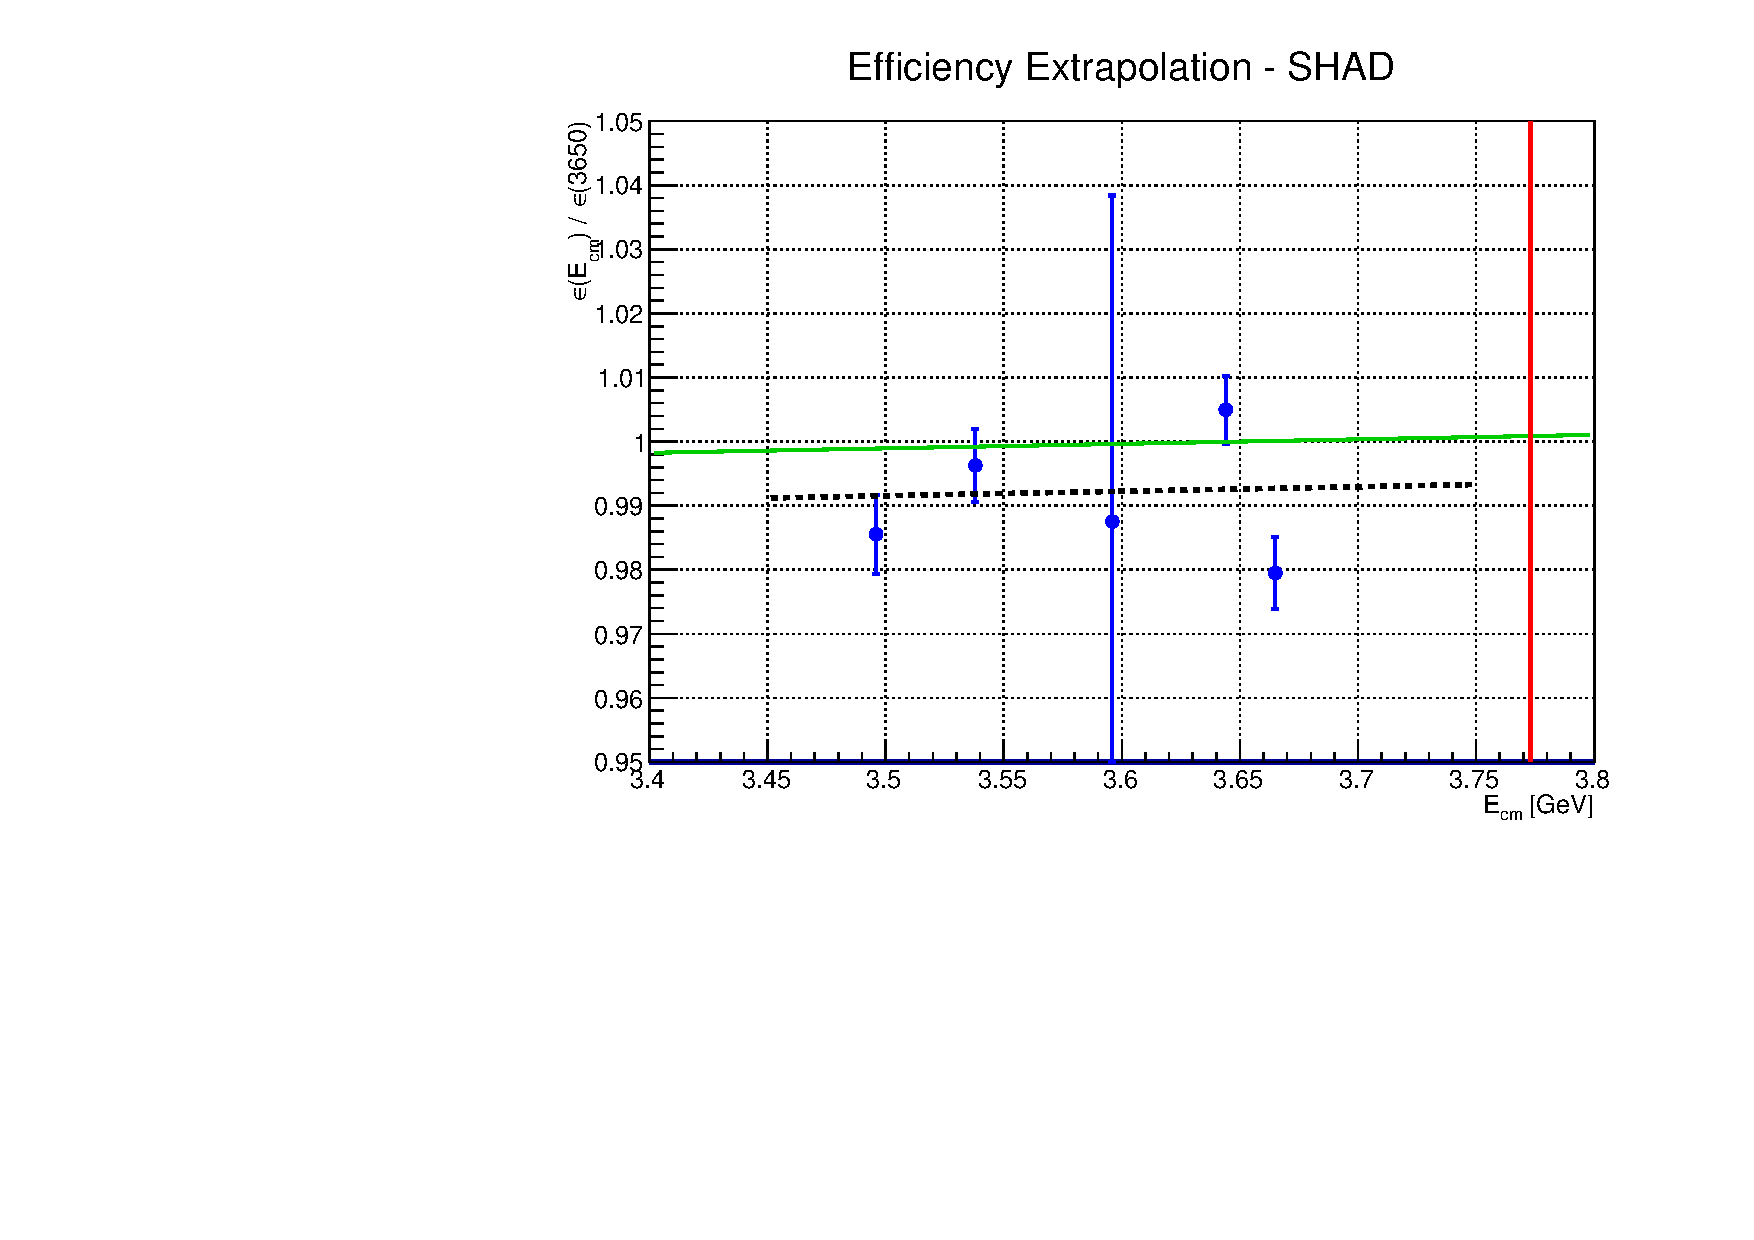
\includegraphics[scale=0.75]{figures/plots/SHAD_psip_BW.pdf}
\caption{The extrapolation for SHAD events using the new continuum data.}
{The new continuum points are fit to a linear slope (dashed black), then extrapolated to higher energies from the old continuum point (solid green). The energy of the $\psipp$ samples (solid red) is also shown.}
\label{fig:extrapolation_SHAD}
\end{figure}

\begin{figure}[H]
\centering
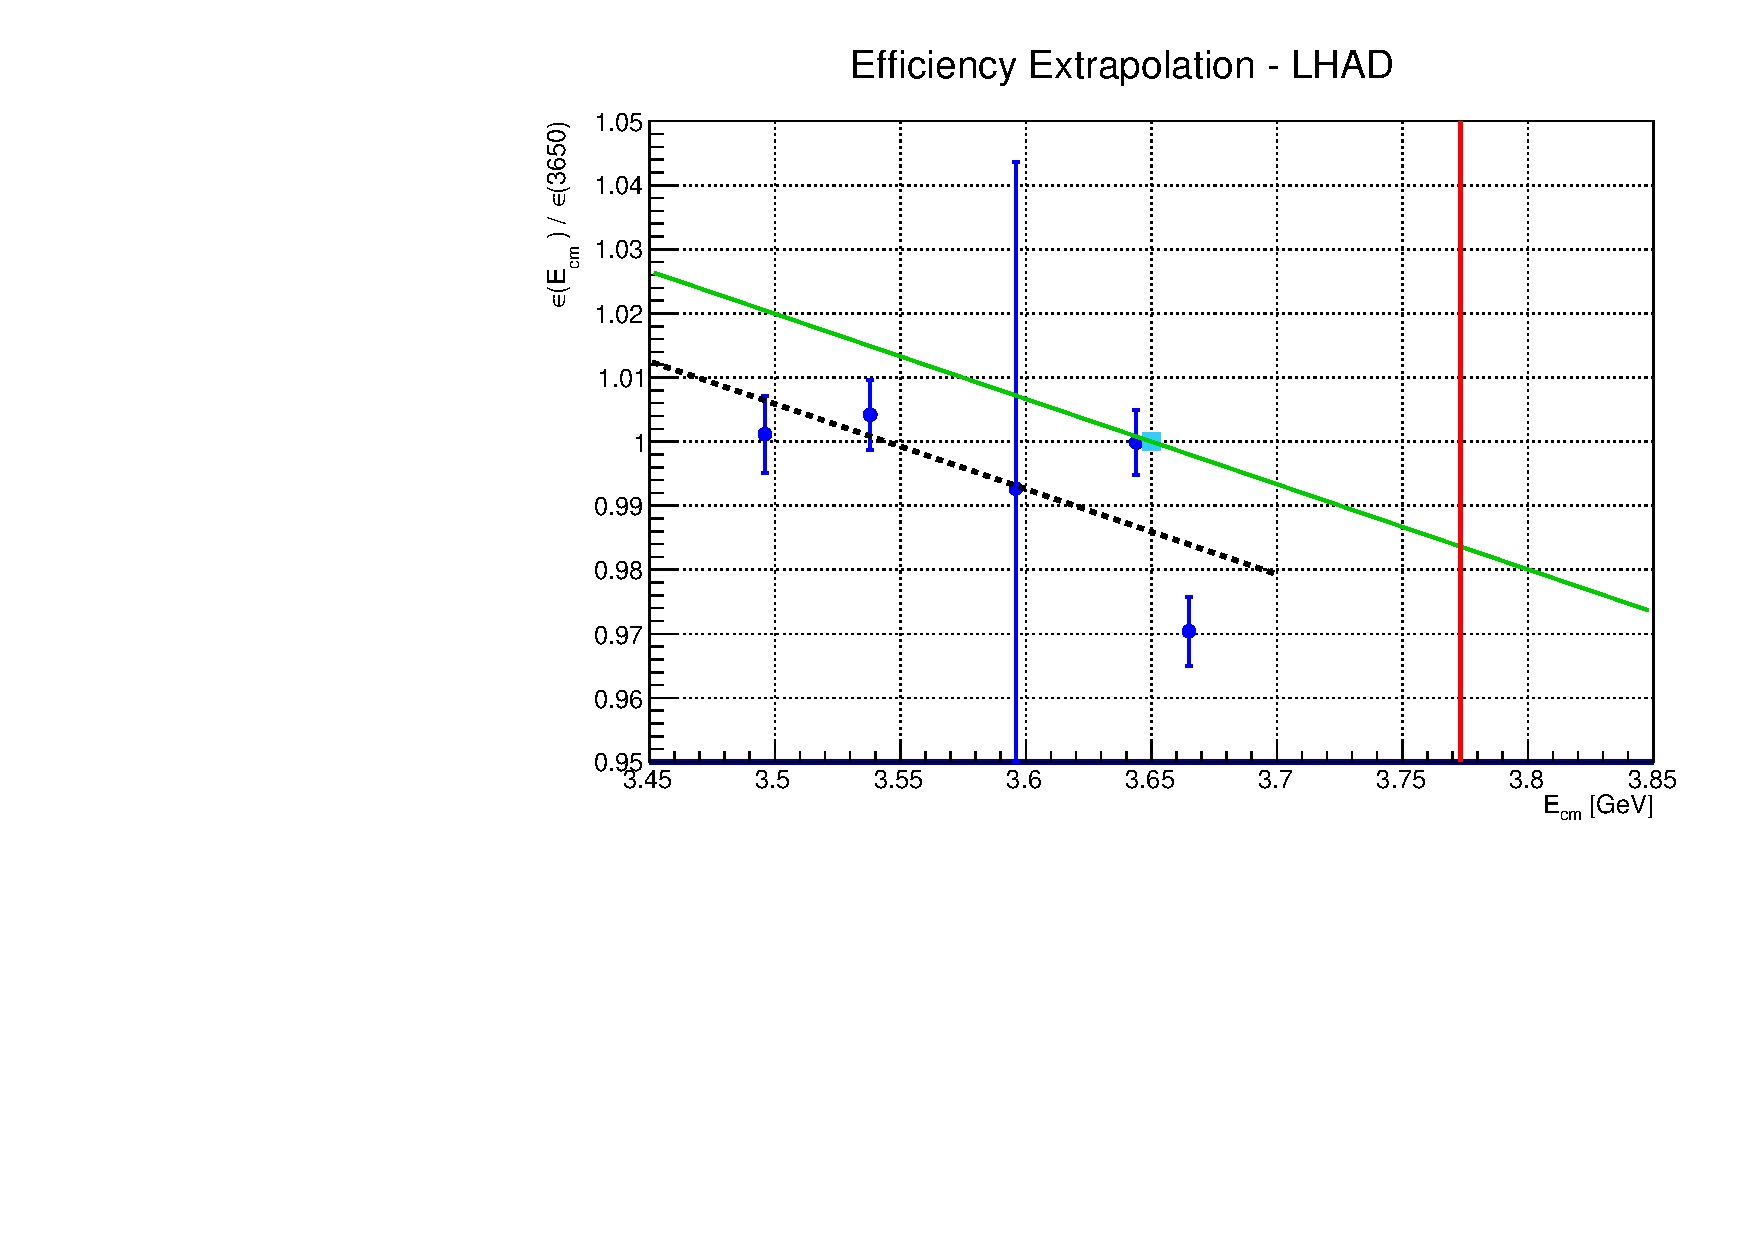
\includegraphics[scale=0.75]{figures/plots/LHAD_psip_BW.pdf}
\caption{The extrapolation for LHAD events using the new continuum data.}
{The new continuum points are fit to a linear slope (dashed black), then extrapolated to higher energies from the old continuum point (solid green). The energy of the $\psipp$ samples (solid red) is also shown.}
\label{fig:extrapolation_LHAD}
\end{figure}

\begin{figure}[H]
\centering
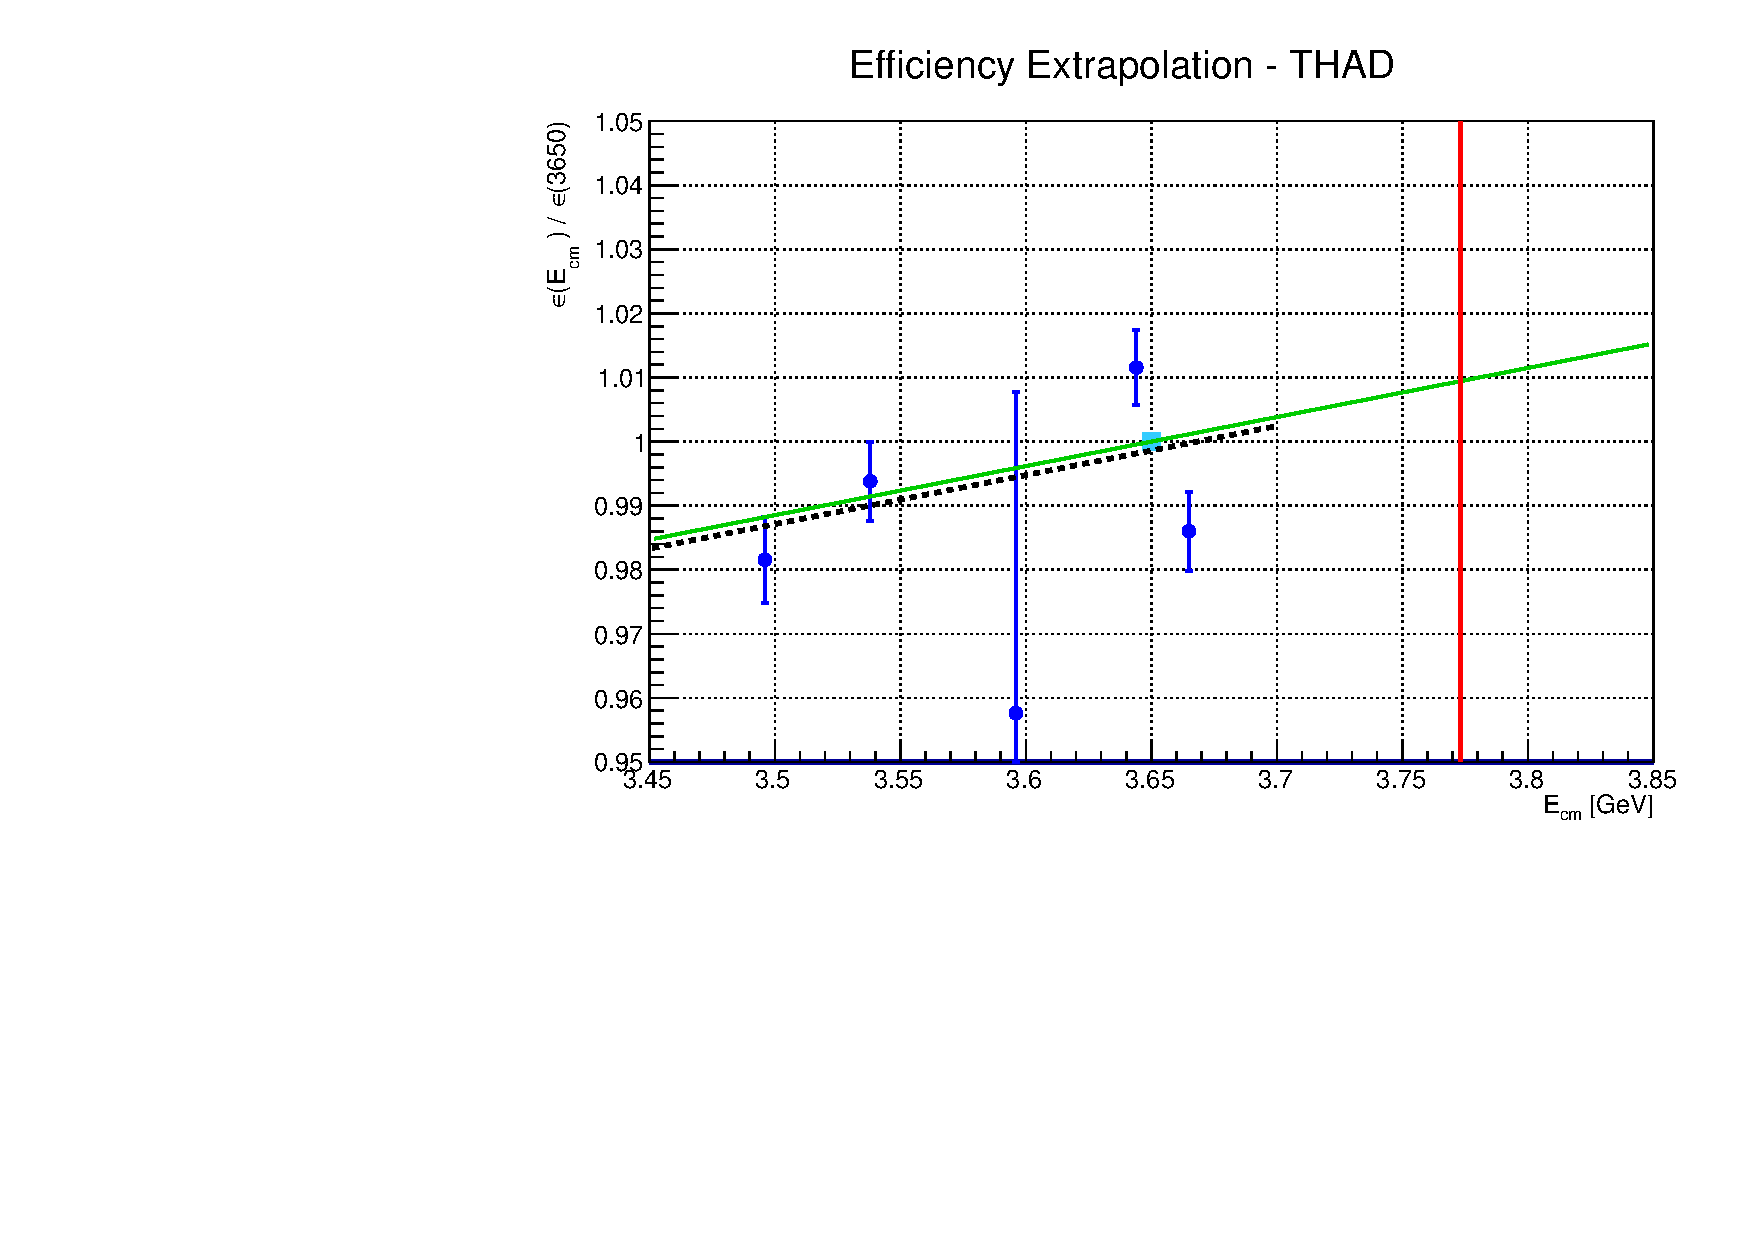
\includegraphics[scale=0.75]{figures/plots/THAD_psip_BW.pdf}
\caption{The extrapolation for THAD events using the new continuum data.}
{The new continuum points are fit to a linear slope (dashed black), then extrapolated to higher energies from the old continuum point (solid green). The energy of the $\psipp$ samples (solid red) is also shown.}
\label{fig:extrapolation_THAD}
\end{figure}



\section{$\DDbar$ Correction}
\label{sec:DDbar_correction}

\section{Results}
\label{sec:non_DDbar_results}
